\documentclass[11pt]{article}
\usepackage[margin=1in]{geometry}
\usepackage[T1]{fontenc}
\usepackage[utf8]{inputenc}
\usepackage{lmodern,microtype,amsmath,amssymb,amsthm,mathtools}
\usepackage{booktabs,graphicx,enumitem,natbib,xcolor,tabularx,array}
\usepackage[colorlinks=true,allcolors=blue!55!black]{hyperref}
\setlist{nosep}
\clubpenalty=10000
\widowpenalty=10000
\displaywidowpenalty=10000
\newcolumntype{Y}{>{\raggedright\arraybackslash}X}
\newcolumntype{P}[1]{>{\raggedright\arraybackslash}p{#1}}
\newtheorem{theorem}{Theorem}
\newtheorem{lemma}{Lemma}
\newtheorem{proposition}{Proposition}
\theoremstyle{remark}
\newtheorem{remark}{Remark}
\newcommand{\R}{\mathbb R}
\newcommand{\E}{\mathbb E}
\newcommand{\PP}{\mathbb P}
\newcommand{\ip}[2]{\langle #1,#2\rangle}
\newcommand{\norm}[1]{\lVert #1\rVert}
\newcommand{\rank}{\operatorname{rank}}
\newcommand{\soft}{\operatorname{soft}}
\newcommand{\TV}{\operatorname{TV}}
\newcommand{\Tu}{\mathrm{Tu}}
\newcommand{\TT}{\mathrm{TT}}
\newcommand{\NL}{\mathrm{NL}}
\newcommand{\calL}{\mathcal L}
\title{Honest Inference for Tensor Contrasts under\newline Tucker and Tensor-Train Rank Bounds}
\author{}
\date{Robustness and adaptation extension: September 11, 2026}

\begin{document}
\maketitle

\begin{abstract}
We study honest confidence intervals for linear functionals of tensor means. Under supplied Tucker or tensor-train rank bounds, the equal-diagonal full-data minimax length is characterized uniformly over positive norm and noise budgets, including arbitrarily weak signals. The corresponding squared-error rate is its square. These upper bounds extend to joint sub-Gaussian errors; directional medians retain the rates over a finite-variance replicate family with a known covariance bound and sufficiently many replicates. A supplied Frobenius approximation allowance adds its size to the interval scale, up to a direct-noise ceiling. For general prescribed loadings we give an orthogonal-surrogate construction with a calibrated residual term, and identify efficiently attained minimax regimes. A growing-rank lower bound and a convex-hull obstruction delimit naive relaxations. At nonzero lower-rank tensors, a shifted mixture illustrates an obstruction from weak additional components. On a different, spectrally separated class, a polynomial SVD/projection procedure selects actual mode ranks without supplied caps and uses an explicit functional-bias certificate. Experiments test its conservatism and failure outside separation, general-loading correction, finite-variance scans, and approximate-rank allowances. Efficient minimax intervals for the original diffuse-loading weak-signal class, sharp geometry for every loading, and general unseparated rank adaptation remain open.
\end{abstract}

\noindent\textbf{Keywords:} honest confidence intervals; linear functionals; Gaussian sequence model; tensor train; Tucker rank; nonconvex parameter space.

\section{Introduction}\label{sec:intro}

Tensor rank models encode restrictions on several unfoldings of the same parameter. For statistical inference, these restrictions are useful only if their effect on interval length survives uncertainty about the actual ranks. A component can be too weak to identify reliably while still belonging to the class over which coverage is required. Consider a third-order $p\times p\times p$ mean tensor $A$ with $\norm A_F\le1$ and rank at most one. From $n=p$ independent full tensors with standard Gaussian errors, the sample mean has noise level $\tau=p^{-1/2}$. The normalized diagonal sum $p^{-1/2}\sum_i A_{iii}$ has a direct interval of length proportional to $\tau$. Can the simultaneous rank restrictions provide a smaller interval with coverage at every admissible mean, including zero?

Existing theory treats several aspects of this question. Tensor functional inference on regular low-rank strata uses accurate subspace estimation and suitable signal conditions \citep{xu2025}. Matrix inference without exact-rank estimation is available under quantitative strength and alignment conditions \citep{choi2026}. Classical work establishes nonlinear functional estimation and the limits of honest adaptation on nonconvex parameter sets \citep{cailownonconvex2004,cailow2004,collier2017}. These precedents motivate a narrower comparison: determine whether joint tensor rank constraints permit a length improvement that cannot be retained by intervals required to cover a larger model defined by a single unfolding.

We study this comparison in the fully observed Gaussian mean experiment, with a known noise variance, a supplied Frobenius bound and supplied upper rank bounds. The loading is a sum of orthogonal product tensors. Honesty means a finite-sample lower bound on coverage over the entire rank-cap class; it includes every lower-rank stratum and every arbitrarily small nonzero singular value. For fixed $K\ge3$, equal mode size $p$ and $M=\tau\sqrt p$, our interval has length $o(\tau)$. By comparison, any honest fixed-radius affine interval on the same class has length at least a constant times $\tau$, and any interval honest over a single-unfolding relaxation has expected length at zero at least a constant times $\tau$. Matricization preserves the data. The latter comparison concerns the parameter space over which coverage is required.

Three mathematical issues govern the argument. Uniform control at rank boundaries requires an envelope that avoids inverses of small singular values. A lower bound for the enlarged model must apply to arbitrary interval procedures, including those using all tensor observations. Finally, optimality depends on which observations a procedure uses: the coordinate diagonal and the full tensor contain different statistical information. This distinction prevents a sharp result for a Gaussian sequence marginal from being mistaken for a sharp full-tensor result.

Canonical Tucker and TT expansions control the sum of squared component weights and hence the $\ell_{2/K}$ size of an orthogonal diagonal. This exponent is familiar from tensor factor geometry \citep{fan2023}. A deterministic error envelope for classical soft thresholding \citep{donohojohnstone1994} then produces an honest interval. Common-target Gaussian mixtures provide the comparison lower bounds. In the third-order example, the radius is at most $\tau\{8\log(2p/\alpha)/p\}^{1/6}$. At rank one, an exact diagonal-image identity permits a specialization of sparse-sequence theory \citep{collier2017}; its lower bound matches this order for diagonal procedures, while full-data analysis requires a different argument. A residual scan exploits off-diagonal information and yields a uniformly short confidence-set projection. A sparse harmonic mixture identifies the larger logarithmic factor in the cubic case. A separate analysis shows that low-degree polynomial estimators need not attain the unrestricted squared-error rate.

The paper develops the following results:
\begin{enumerate}
\item An explicit diagonal envelope for Tucker and TT cap classes, and a finite-sample interval valid across their lower-rank strata (Sections~\ref{sec:method}--\ref{sec:theory}).
\item Two quantitative separations: from fixed-radius affine intervals under the same honesty class, and from all intervals under a single-unfolding relaxation (Section~\ref{sec:theory}).
\item Sharp full-data minimax expected length, both at zero and in the worst case, with rates depending on whether $K=3$ or $K\ge4$; the corresponding squared-error rates (Section~\ref{sec:sharp_full}).
\item An explicit truncated-scan computation tradeoff and a low-degree polynomial estimation obstruction, distinguished from a lower bound for every efficient confidence interval (Section~\ref{sec:computation}).
\item A full norm-budget phase diagram, a residual-fit squared-risk theorem, and loading-dependent bounds with matching flat-support rates (Section~\ref{sec:norm_loading}).
\item Full-data robust-noise and approximate-rank extensions; certified general-loading and efficient regimes; an adaptation obstruction and a separated rank-calibrated procedure with new experiments (Section~\ref{sec:robust_adaptive}).
\end{enumerate}

\section{Related work}\label{sec:related}

\paragraph{Gaussian functionals and approximate sparsity.}
Optimal recovery and nonconvex functional estimation connect risk to the geometry of the parameter set \citep{donoho1994,cailownonconvex2004}. In the Gaussian sequence model $y=\theta+\sigma g$, \citet{collier2017} give sharp rates for $\sum_i\theta_i$ over $\ell_q$ balls. In their sparse regime, the squared-error scale is
\[
 \sigma^2(r/\sigma)^{2q}
 \{\log[1+d(\sigma/r)^{2q}]\}^{1-q},
 \qquad \norm\theta_q\le r,\quad 0<q\le1.
\]
The specialization $q=2/K$, $r=M=\tau\sqrt p$, $d=p$ and division by $p$ for our normalized contrast yields the squared diagonal-information rate below. We explicitly credit this benchmark and give its confidence-interval derivation. Its transfer to the full tensor experiment would require a different lower bound. Our full-data scan and harmonic mixture provide separate arguments in that experiment.

\paragraph{Honest adaptation and weak ranks.}
The confidence-interval theory of \citet{cailow2004} uses between-class moduli and testing to characterize adaptation, while \citet{low1997} gives foundational limitations. Finite convex-union aggregation is developed by \citet{juditskynemirovski2020}. Thus, neither nonlinear inference nor failure of uniform adaptation at a model boundary is peculiar to tensors. Matrix confidence sets and detection results further show that attainable rank adaptation depends on the observation design and loss \citep{carpentieretal2018,carpentiernickl2015}.

In econometric models, \citet{choi2026} study $Y_{it}=X_{it}M_{it}+E_{it}$ and construct studentized block-average inference with a projection dimension at least the true rank. Their quantitative strength and alignment assumptions remain relevant even though exact rank is not estimated. \citet{armstrong2026} consider a regression coefficient in a panel with a low-rank interactive effect, using weights and a bias bound for uniform inference without a minimum factor strength. \citet{zhu2019} establishes weak-factor and rank-adaptation obstructions in a missing-entry experiment. These are different targets and designs from the fully observed tensor contrast considered here.

\paragraph{Regular matrix and tensor functional inference.}
For tensor regression $Y_i=\ip{X_i}A+\epsilon_i$, \citet{xu2025} combine a pilot estimator with debiasing and tangent projection to infer general linear functionals. Their regular-stratum results require rank/subspace control and signal/remainder conditions; the principal regression theorem imposes a positive minimum unfolding signal. Its tangent standard deviation is of the form $\sigma\norm{P_{T_A}L}_F/\sqrt n$. Our replacement is uniform finite-sample coverage on a cap union, at the cost of a narrower loading, known norm/noise bounds and potentially conservative length. No pointwise dominance over that efficient regime is asserted.

Related matrix linear-form inference, geometric inverse-problem inference and limiting distributions under rank caps are developed by \citet{xiayuan2021,cailiangrakhlin2016,carpentierkim2018}. Tensor subspace and functional inference includes strong-signal results of \citet{xiazhangzhou2022,agterberg2024}; \citet{caipoorchen2023} treats tensor completion and entry/factor uncertainty. Covariance-weighted low-rank regression inference \citep{ke2026} and uniform inference for weak matrix signals \citep{bykhovskaya2025} provide recent neighboring results. Their observation models and regularity conditions cannot be replaced by the Gaussian location experiment without proof.

\citet{madu2026} also give a tensor-completion confidence-length lower bound in their Theorem 10. Its class imposes incoherence, a positive minimum unfolding signal, a condition-number cap and nonvanishing tangent-loading alignment. It excludes zero and uses randomly sampled entries; it does not supply a lower bound for the rank-boundary Gaussian location problem here.

\paragraph{Computational restrictions.}
Low-degree likelihood methods provide restricted computational lower bounds for sparse tensor PCA \citep{choo2021}. Recent work further studies low-degree estimation thresholds for planted hypergraphs and tensor PCA \citep{fu2026}. Our coarse overlap-moment argument is self-contained and targets the scalar contrast; it does not claim that low-degree polynomials represent every efficient algorithm.

\paragraph{Geometry and finite-sample inference.}
Orthonormal Tucker and TT representations are standard \citep{delathauwer2000,oseledets2011}. Tensor norms and Euclidean factor penalties already contain the exponent $2/K$ \citep{friedlandlim2018,fan2023}; tangent cones of Tucker and TT varieties have also been studied \citep{gao2025,kutschan2018}. We use canonical expansions without estimating tangent spaces. Singular-model likelihood theory \citep{drton2009} and universal inference \citep{wasserman2020} establish broader approaches to nonregular validity. Our specific comparison concerns interval length under simultaneous rank constraints, rather than generic existence of a valid interval.

The comparison can be written as
\[
 \text{regular-stratum functional inference}
 \quad\longrightarrow\quad
 \text{cap-uniform inference for a restricted loading},
\]
and, within the present Gaussian experiment,
\[
 \text{honesty on one unfolding class}
 \ \longrightarrow\
 \text{honesty on the joint tensor class}.
\]
The first changes assumptions and loading scope; the second permits a quantitative length separation. The companion survey records 20 closest papers and their mathematical differences, including relevant work available by September 9, 2026.

\section{Experiment and parameter classes}\label{sec:model}

Let $K\ge2$, $p_k\ge1$, and $D=\prod_{k=1}^K p_k$. We observe
\begin{equation}\label{eq:model}
 Z=A+\tau G\in\R^{p_1\times\cdots\times p_K},\qquad
 \operatorname{vec}(G)\sim N(0,I_D),\qquad \tau>0.
\end{equation}
The noise level is known in the baseline model. Section~\ref{sec:robust_adaptive} states different, explicitly calibrated noise and rank assumptions. Equivalently, $Z$ is the sufficient sample mean of independent full observations $W_j=A+\sigma G_j$, $j=1,\ldots,n$, with known $\sigma$ and $\tau=\sigma/\sqrt n$. This is an exact Gaussian mean equivalence, not an equivalence to scalar-response tensor regression. The observed variables are the tensors $W_j$, or $Z$; $A$ is a fixed unknown parameter. Factor and core representations are nonunique coordinates, not additional latent random variables.

Write $A_{(k)}$ for the mode-$k$ unfolding and $A_{\langle k\rangle}$ for the matrix joining modes $1,\ldots,k$ against $k+1,\ldots,K$. For supplied positive integer caps, define
\begin{align}
 \Theta_{\Tu}(M,\bar r)&=\{A:\norm A_F\le M,\ \rank(A_{(k)})\le\bar r_k,\ k=1,\ldots,K\},\label{eq:tucker}\\
 \Theta_{\TT}(M,\bar r)&=\{A:\norm A_F\le M,\ \rank(A_{\langle k\rangle})\le\bar r_k,\ k=1,\ldots,K-1\}.\label{eq:tt}
\end{align}
The known bound $M$ is positive. Actual ranks may be smaller, including zero; nonzero singular values may be arbitrarily small. No incoherence or coordinate sparsity condition is imposed. The main experiment assumes Gaussian isotropic noise and exact caps. Appendix~\ref{app:refinements} states separately calibrated noise and approximation extensions; missing observations remain untreated.

The prescribed loading has the form
\begin{equation}\label{eq:loading}
 L=\sum_{i=1}^m w_i V_i,\qquad
 V_i=\bigotimes_{k=1}^K v_{ki},\qquad
 v_{ki}^\top v_{kj}=\mathbf1\{i=j\},\qquad \norm w_2=1.
\end{equation}
Here $m\le\min_k p_k$, and each loading family is supplied independently of the data. Thus $\norm L_F=1$. Although this is restrictive, $L$ need not be sparse in the observation basis: known orthogonal mode rotations can make it dense. The estimand and relevant observations are
\begin{equation}\label{eq:diagonal}
 \psi(A)=\ip LA=\sum_iw_i a_i,\qquad
 a_i=\ip A{V_i},\qquad d_i=\ip Z{V_i}=a_i+\tau g_i,
\end{equation}
where the $g_i$ are independent standard normals.

An interval $C(Z)$ is honest at level $1-\alpha$ on $\Theta$ if
\begin{equation}\label{eq:honesty}
 \inf_{A\in\Theta}\PP_A\{\psi(A)\in C(Z)\}\ge1-\alpha.
\end{equation}
This is a finite-sample requirement, not a pointwise limit along a fixed-rank stratum. Length and expected length are the primary criteria. For example,
\begin{equation}\label{eq:minimaxcriteria}
 \calL_0(\Theta)=\inf_{C:\,\eqref{eq:honesty}}\E_0|C|,
 \qquad \calL_{\max}(\Theta)=\inf_{C:\,\eqref{eq:honesty}}\sup_{A\in\Theta}\E_A|C|.
\end{equation}
The infima range over all measurable intervals, allowing independent randomization. The usual squared Frobenius estimation loss has population risk $R_A(B)=\norm{B-A}_F^2+D\sigma^2$ and empirical risk $R_n(B)=n^{-1}\sum_j\norm{W_j-B}_F^2$. We do not minimize these risks or require a full-tensor estimator.

The principal asymptotic comparison in experiment~\eqref{eq:model} uses $p_k=m=p$, fixed $K\ge3$, fixed rank caps, and $M=\tau\sqrt p$. A concrete sequence is $M=\sigma=1$, $n=p$, so $D=n^K$. Section~\ref{sec:norm_loading} removes the relation between $M$ and $\tau$ for the sharp full-data results and extends them to flat orthogonal loadings in unequal ambient dimensions.


The structural and probabilistic assumptions have distinct roles, summarized in Table~\ref{tab:assumptions}. A1--A4 define the inferential problem; A5 is used for the original asymptotic comparisons. The norm/noise relation in A5 is not required in Section~\ref{sec:norm_loading}.
\begin{table}[ht]
\centering\small
\begin{tabularx}{\textwidth}{@{}lYY@{}}
\toprule
 & Assumption & Role and restriction \\
\midrule
A1 & Full observation with independent Gaussian coordinates and known $\tau$ & Gives exact diagonal noise, direct calibration and Gaussian likelihood identities. \\
A2 & Supplied $M$ and Tucker or TT upper rank bounds & Defines the outer honesty class; actual rank and signal strength are unrestricted below it. \\
A3 & Prescribed loading in \eqref{eq:loading} & Gives orthogonal noise coordinates and the diagonal envelope; data-selected loadings are excluded; arbitrary prescribed loadings are treated separately in Section~\ref{sec:robust_adaptive}. \\
A4 & Finite-sample uniform coverage in \eqref{eq:honesty} & Coverage includes zero and local sequences approaching lower-rank strata. \\
A5 & Equal dimensions, fixed $K\ge3$, fixed caps and $M=\tau\sqrt p$ & Produces the stated vanishing length ratio; not needed for the finite-sample interval. \\
\bottomrule
\end{tabularx}
\caption{Assumptions, their purpose and the scope they exclude. Known upper bounds are not replaced by same-data estimates anywhere in the stated procedure.}
\label{tab:assumptions}
\end{table}

\section{Interval construction}\label{sec:method}

Define
\begin{equation}\label{eq:constants}
 q=\frac2K,\quad
 J_{\Tu}=\min_k\prod_{\ell\ne k}\bar r_\ell,\quad
 J_{\TT}=\prod_{k=1}^{K-1}\bar r_k,\quad B=J^{1-q/2}M^q,
\end{equation}
where $J$ is chosen for the applicable class. Set
\begin{equation}\label{eq:threshold}
 \lambda=\tau\sqrt{2\log(2m/\alpha)},\qquad
 \widehat\psi_{\NL}=\sum_iw_i\soft_\lambda(d_i),\qquad
 \soft_\lambda(x)=\operatorname{sign}(x)(|x|-\lambda)_+.
\end{equation}
The three candidate intervals have radii
\begin{align}
 h_{\NL}&=\norm w_\infty B(2\lambda)^{1-q},&
 I_{\NL}&=[\widehat\psi_{\NL}-h_{\NL},\widehat\psi_{\NL}+h_{\NL}],\label{eq:nl}\\
 h_G&=z_{1-\alpha/2}\tau,&
 I_G&=[\ip LZ-h_G,\ip LZ+h_G],\label{eq:direct}\\
 h_0&=M\left(\sum_{i=1}^s w_{(i)}^2\right)^{1/2},&
 I_0&=[-h_0,h_0],\label{eq:zero}
\end{align}
where $|w_{(1)}|\ge\cdots\ge|w_{(m)}|$ and $s$ is the smaller of $m$ and the smallest supplied rank cap. Choose
\begin{equation}\label{eq:select}
 C_*=I_{j_*},\qquad j_*\in\arg\min_{j\in\{\NL,G,0\}}h_j,
\end{equation}
with a fixed rule for ties. This choice depends only on known quantities. Choosing an interval after examining its center or an estimated rank is a different procedure and is not justified by the proof.

The constants in \eqref{eq:constants} calibrate the threshold procedure~\eqref{eq:threshold}; the direct alternative~\eqref{eq:direct} supplies a valid fallback. Only $m$ contractions are used. For coordinate loadings, computation reads $m$ tensor entries and takes $O(m)$ operations. Obtaining contractions for a dense rotated loading has additional cost, which can be large. The procedure does not estimate a Tucker core, TT cores, factors or actual ranks.

\section{Statistical theory}\label{sec:theory}

All numbered theorems and propositions are \textbf{PROVED}, with complete derivations in the appendix. The result-status table separates the proved statements from open computational and adaptive questions. The results use the experiment and classes of Section~\ref{sec:model}. Lower-bound constants are stated for $0<\alpha<1/4$ when this simplifies positivity.

\subsection{Diagonal geometry and honest coverage}

\begin{theorem}[Orthogonal diagonal compressibility]\label{thm:diagonal}
For either class in \eqref{eq:tucker}--\eqref{eq:tt}, under loading \eqref{eq:loading},
\begin{equation}\label{eq:compress}
 \sum_{i=1}^m|\ip A{V_i}|^{2/K}\le J^{1-1/K}M^{2/K}.
\end{equation}
No minimum singular value is required.
\end{theorem}

The proof expands a canonical tensor representation into at most $J$ product terms whose squared component weights sum to $\norm A_F^2$. For TT tensors, these terms need not be orthogonal. A prefix-weight identity establishes the sum exactly; assuming termwise orthogonality would be an incorrect shortcut. H\"older's inequality and Bessel's inequality then give \eqref{eq:compress}. The rank factor may be loose, particularly for growing caps.

For rank cap one the diagonal image is exactly the ball $\{a:\sum_i|a_i|^{2/K}\le M^{2/K}\}$, as shown in Lemma~\ref{lem:image}. Thus the diagonal-only statistical experiment is precisely a classical Gaussian sequence problem on an $\ell_q$ ball. The full tensor experiment contains additional off-diagonal information. This identity permits a sharp benchmark for the restricted observation experiment; it does not remove the additional information in the rest of the tensor.

\begin{theorem}[Finite-sample honest interval]\label{thm:coverage}
For every $0<\alpha<1$, each interval in \eqref{eq:nl}--\eqref{eq:zero} is honest on the applicable cap class. Consequently, $C_*$ is honest and has deterministic length
\begin{equation}\label{eq:length}
 |C_*|=2\min\{h_{\NL},h_G,h_0\}.
\end{equation}
\end{theorem}

The event $\max_i|\tau g_i|\le\lambda$ has probability at least $1-\alpha$. On this event soft thresholding satisfies
\[
 |\soft_\lambda(a_i+\tau g_i)-a_i|\le\min(|a_i|,2\lambda)
 \le |a_i|^q(2\lambda)^{1-q}.
\]
Summing proves the nonlinear interval bound. No central limit theorem, rank recovery or pilot remainder is needed. Known $M$ is essential to this deterministic calibration.

\subsection{Two lower-bound comparisons}

For the remainder of this subsection let all dimensions equal $p$, let $E_i=e_i^{\otimes K}$, and put
\begin{equation}\label{eq:equalL}
 L=p^{-1/2}\sum_{i=1}^p E_i,\qquad z=z_{1-\alpha/2}.
\end{equation}

\begin{theorem}[Fixed-radius affine intervals]\label{thm:affine}
Suppose the honesty class contains $0$ and all $\pm M E_i$. If $0<\alpha<1/2$ and
\[
 C(Z)=[\ip WZ+b-h,\ip WZ+b+h]
\]
is honest, with deterministic $W,b,h$, then
\begin{equation}\label{eq:affinelower}
 h\ge\frac{(M/\sqrt p)z\tau}{M/\sqrt p+z\tau}.
\end{equation}
On the rank-one tensor Frobenius ball, the best radius in this affine class is therefore of order $\min(M/\sqrt p,\tau)$, up to constants depending on $\alpha$.
\end{theorem}

The theorem allows $W$ to use the entire tensor. It does not cover affine centers with data-dependent radii. The matching upper order follows by choosing between $I_G$ and $I_0$ for rank cap one.

For a nonempty proper subset $S$ of modes, write $A_{[S]}$ for the corresponding bipartition unfolding and define
\begin{equation}\label{eq:relax}
 \Theta_S=\{A:\rank(A_{[S]})\le1,\ \norm A_F\le M\}.
\end{equation}

\begin{theorem}[Cost of a single unfolding honesty class]\label{thm:unfolding}
If $0<\alpha<1/4$, every interval honest on $\Theta_S$ satisfies
\begin{equation}\label{eq:unfoldlower}
 \E_0|C|\ge c_\alpha\min\left\{\frac M{\sqrt p},\frac\tau4\right\},\qquad
 c_\alpha=1-2\alpha-\frac12\sqrt{\sqrt{8/7}-1}>0.
\end{equation}
The lower order $\min(M/\sqrt p,\tau)$ is attained up to $\alpha$-dependent constants by the direct/structural choice on $\Theta_S$.
\end{theorem}

The alternatives in the proof are rank one in the chosen matrix unfolding. They generally violate the other tensor rank constraints. This is necessary for the comparison: the theorem measures the cost of requiring coverage on the larger class. For Tucker caps, a mode unfolding is a permissible relaxation; for TT caps, a contiguous cut is permissible. With all tensor rank caps one, every bipartition in \eqref{eq:relax} contains the original tensor class. Increasing an unfolding cap further preserves the lower bound.

\begin{theorem}[Strict length separations]\label{thm:separation}
Let $0<\alpha<1/4$, $K\ge3$ and the rank caps be fixed. Under \eqref{eq:equalL} and $M=\tau\sqrt p$, $C_*$ is honest on the Tucker or TT class and
\begin{equation}\label{eq:separation}
 |C_*|\le2\tau J^{1-1/K}
 \left\{\frac{8\log(2p/\alpha)}p\right\}^{(K-2)/(2K)}=o(\tau).
\end{equation}
In contrast, every fixed-radius affine interval honest on the same class has length at least $2z\tau/(1+z)$. Every interval honest on a class retaining only one constrained unfolding has expected length at zero at least $c_\alpha\tau/4$.
\end{theorem}

For growing caps, the same conclusion follows if $J^{1-1/K}(\log p/p)^{(K-2)/(2K)}\to0$. This condition may be restrictive. At $K=2$ the exponent in \eqref{eq:separation} is zero, so the argument gives no polynomial separation. Theorem~\ref{thm:separation} neither asserts that the displayed exponent is optimal nor compares favorably at every strong signal with an efficient oracle projection interval. Figure~\ref{fig:theory} displays the explicit comparisons and the within-class bracket established next.

\subsection{An initial full-data lower bound}\label{sec:gap}

\begin{theorem}[Within-class lower bound]\label{thm:jointlower}
Under \eqref{eq:model} and \eqref{eq:equalL}, for $0<\alpha<1/4$, every interval honest on a class containing the rank-one tensor Frobenius ball of radius $M$ satisfies
\begin{equation}\label{eq:jointlower}
 \E_0|C|\ge(3/4-2\alpha)
 \frac{\min\{M,\tau\sqrt{\log(1+p/4)}\}}{\sqrt p}.
\end{equation}
\end{theorem}

This is a sparse-coordinate mixture bound. At $M=\tau\sqrt p$, for fixed caps and fixed $K\ge3$, the results imply
\begin{equation}\label{eq:gap}
 c\tau\sqrt{\frac{\log p}p}
 \le\calL_0(\Theta)\le\calL_{\max}(\Theta)
 \le C\tau\left(\frac{\log p}p\right)^{(K-2)/(2K)}
\end{equation}
for sufficiently large $p$, with constants depending on $K$, the caps and $\alpha$. The ratio of these initial scales grows as $(p/\log p)^{1/K}$. Section~\ref{sec:sharp_full} closes the gaps: the two criteria in \eqref{eq:minimaxcriteria} have the same rate, with an additional logarithmic factor in the cubic case.

\subsection{Optimality when only the diagonal is observed}\label{sec:diagonal_optimality}

Let $\Theta_1$ denote the Frobenius ball of tensors with rank at most one, including zero. Restrict the interval to be measurable in $d=(Z_{i,\ldots,i})_{i=1}^p$ and an independent random seed. Write $\mathcal C_{\alpha,d}(\Theta_1)$ for such intervals that are honest on $\Theta_1$, and define
\[
 \mathcal L_{0,d}(\Theta_1)=\inf_{C\in\mathcal C_{\alpha,d}(\Theta_1)}\E_0|C|,
 \qquad
 \mathcal L_{\max,d}(\Theta_1)
 =\inf_{C\in\mathcal C_{\alpha,d}(\Theta_1)}\sup_{A\in\Theta_1}\E_A|C|.
\]
The next result specializes classical sparse-sequence arguments \citep{cailownonconvex2004,collier2017} to honest intervals. It is a benchmark for the proposed use of diagonal information, not a new Gaussian-sequence minimax principle.

\begin{proposition}[Classical diagonal-information benchmark]\label{prop:diagonal_minimax}
Assume \eqref{eq:model}, \eqref{eq:equalL} and $0<\alpha<1/4$. For each integer $1\le s\le p$, put
\[
 b_s=\min\left\{M s^{-K/2},\
       \tau\sqrt{\log\left(1+\frac{p}{4s^2}\right)}\right\},
 \qquad
 c_{\alpha,d}=1-2\alpha-\frac12\sqrt{e^{1/4}-1}>0.
\]
Every $C\in\mathcal C_{\alpha,d}(\Theta_1)$ satisfies
\begin{equation}\label{eq:diagonal_lower}
 \E_0|C|\ge c_{\alpha,d}\frac{s b_s}{\sqrt p}.
\end{equation}
For fixed $K\ge3$ and $M=\tau\sqrt p$,
\begin{equation}\label{eq:diagonal_rate}
 \mathcal L_{0,d}(\Theta_1)\asymp
 \mathcal L_{\max,d}(\Theta_1)\asymp
 \tau\left(\frac{\log p}{p}\right)^{(K-2)/(2K)}.
\end{equation}
The comparison constants depend on $K$ and $\alpha$.
\end{proposition}

The rate in \eqref{eq:diagonal_rate} follows because the effective support size $s\asymp(p/\log p)^{1/K}$ makes \eqref{eq:diagonal_lower} match the threshold interval's upper order. The same asymptotic conclusion holds for any fixed Tucker or TT caps: the class contains $\Theta_1$ and Theorem~\ref{thm:coverage} changes the upper bound only by a fixed rank factor. Thus further improvement in the power of $p$ cannot come from recalibrating a procedure restricted to $d$.

This result does not close the full-data gap in \eqref{eq:gap}. For the common-target tensors $A_S=b_s(\sum_{i\in S}e_i)^{\otimes K}$, two support sets with overlap $J$ have diagonal inner product $b_s^2J$ but full-tensor inner product $b_s^2J^K$. The likelihood second moment in the full experiment is consequently different. A valid diagonal lower bound cannot be transferred by ignoring the extra observations. Theorem~\ref{thm:scan} establishes that they do permit shorter expected length at zero.

Table~\ref{tab:theory_comparison} separates the procedure and parameter classes in the comparisons; Figure~\ref{fig:theory} displays the corresponding bounds.
\begin{table}[ht]
\centering\small
\begin{tabularx}{\textwidth}{@{}P{0.24\textwidth}P{0.22\textwidth}Y@{}}
\toprule
Comparison & Information and honesty class & Length statement when $M=\tau\sqrt p$ \\
\midrule
Direct Gaussian interval & All means; prescribed $L$ & $2z\tau$, with exact coverage. \\
Selected interval & Joint cap class; uses $d$ & At most $2\tau J^{1-1/K}\{8\log(2p/\alpha)/p\}^{\beta}$; $\beta=(K-2)/(2K)$. \\
Any fixed-radius affine interval & Full tensor; same joint class & Length at least $2z\tau/(1+z)$. \\
Any interval on one unfolding class & Full tensor; enlarged honesty class & Expected length at zero at least $c_\alpha\tau/4$. \\
Any diagonal-based interval & Only $d$; rank-one or fixed-cap class & Optimal expected length at zero and in worst case has order $\tau(\log p/p)^\beta$. \\
Any full-data interval & Full tensor; joint class & Optimal expected length both at zero and in the worst case is $r_K(p)$ in \eqref{eq:full_rates}. \\
\bottomrule
\end{tabularx}
\caption{Precisely delimited comparisons for fixed $K\ge3$ and fixed rank caps. Lower bounds for relaxed honesty classes or restricted observations are not lower bounds for unrestricted full-data procedures on the original class.}
\label{tab:theory_comparison}
\end{table}

\begin{figure}[t]
\centering
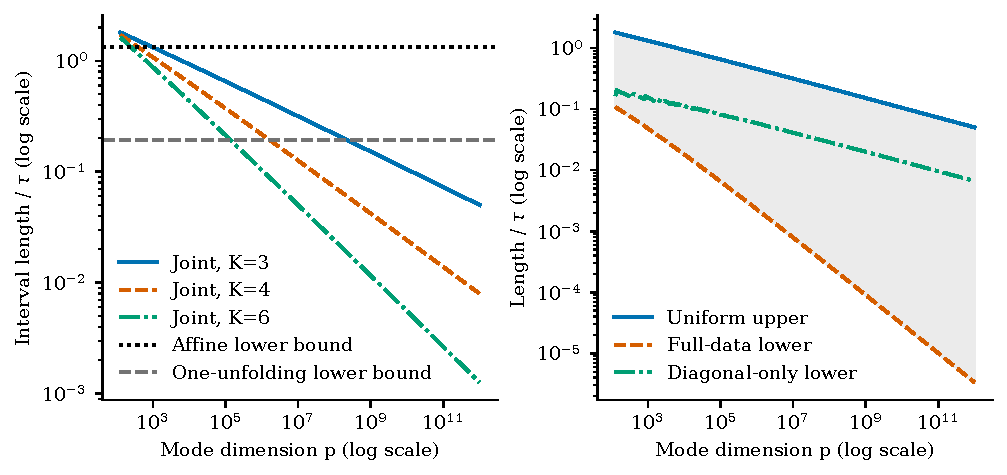
\includegraphics[width=\textwidth]{figures/theoretical_comparison.pdf}
\caption{Joint constraints permit vanishing normalized length, and the diagonal-only lower bound matches its order. Left: cap-one selected length and the affine and one-unfolding lower bounds, for $M=\tau\sqrt p$ and $\alpha=0.05$. Right: the $K=3$ upper bound, the full-data lower bound and the diagonal-only lower bound from \eqref{eq:diagonal_lower}, using $s=\lfloor(p/\log p)^{1/3}\rfloor$. The right panel shows the initial bounds, before the improvements in Theorems~\ref{thm:scan}--\ref{thm:full_minimax}; it is not the final full-data bracket. Curves evaluate analytic formulas up to $p=10^{12}$; simulated dimensions stop at $8192$.}
\label{fig:theory}
\end{figure}


\subsection{Using the full tensor at the zero mean}\label{sec:full_scan}

The diagonal rate is a constraint on procedures using the diagonal. A finite scan over product directions of coordinate subtensors can give shorter expected length at zero while preserving the original uniform length bound. The scan is an existence construction with exponential complexity; no efficient implementation is asserted.

For a tensor $B$, define its injective norm
\[
 \rho(B)=\sup_{\norm{u_k}_2=1}
       |\ip B{u_1\otimes\cdots\otimes u_K}|.
\]
For every nonempty subset $S\subseteq\{1,\ldots,p\}$ of size $s$, choose fixed $1/(2K)$-nets of the unit sphere in $\R^s$, one per mode, each with at most $(1+4K)^s$ points. Let $N_S(Z)$ be the largest absolute contraction of $Z_{S,\ldots,S}$ over their product. Define
\begin{align}
 \lambda_s^{\rm scan}
 &=\tau\left[2\{s\log(ep/s)+Ks\log(1+4K)+\log(2p/\gamma)\}\right]^{1/2},
 \label{eq:scan_threshold}\\
 R_\gamma
 &=\frac{4J^{K/2}}{\sqrt p}
       \sum_{s=1}^p\lambda_s^{\rm scan}s^{-K/2}.
 \label{eq:scan_radius}
\end{align}
Accept the zero test if $N_S(Z)\le\lambda_{|S|}^{\rm scan}$ for every nonempty $S$. On acceptance, let $C_{\rm scan}=[-h_{\rm scan},h_{\rm scan}]$, where $h_{\rm scan}=\min(h_0,R_\gamma)$; on rejection let $C_{\rm scan}=[-h_0,h_0]$. Here $h_0=M\sqrt{s_{\rm cap}/p}$ and $s_{\rm cap}$ is the smallest cap, truncated at $p$. For $0<\alpha_0,\gamma<1$ with $\alpha_0+\gamma\le\alpha$, intersect this interval with $C_*(\alpha_0)$ and call the result $C_\dagger$; replace an empty intersection by $\{0\}$. Write $\ell_*=|C_*(\alpha_0)|$.

\begin{theorem}[A full-data interval with short expected length at zero]\label{thm:scan}
Under \eqref{eq:model}, \eqref{eq:equalL} and either cap class, $C_{\rm scan}$ is honest at level $1-\gamma$, and $C_\dagger$ is honest at level $1-\alpha$. Moreover,
\begin{equation}\label{eq:scan_expectation}
 \sup_{A\in\Theta}\E_A|C_\dagger|\le\ell_*,
 \qquad
 \E_0|C_\dagger|\le
 \min\{\ell_*,\,2R_\gamma+\ell_*\gamma\}.
\end{equation}
For fixed $0<\alpha<1/4$, fixed $K\ge3$, fixed positive caps and $M=\tau\sqrt p$, choose $\alpha_0=\alpha/2$ and $\gamma=\alpha/(2p)$. Then
\begin{equation}\label{eq:scan_rate}
 \E_0|C_\dagger|
 \le C_{K,J,\alpha}\frac{\tau\sqrt{\log p}}{\sqrt p}
       \sum_{s=1}^p s^{-(K-1)/2}
\end{equation}
for sufficiently large $p$. Consequently,
\begin{equation}\label{eq:zero_sharp}
 \calL_0(\Theta)\asymp\tau\sqrt{\frac{\log p}{p}},
 \qquad K\ge4.
\end{equation}
\end{theorem}

The matching lower bound in \eqref{eq:zero_sharp} is Theorem~\ref{thm:jointlower}, applied to the same full-data experiment and honesty class. The sum in \eqref{eq:scan_rate} is bounded for $K\ge4$ and harmonic for $K=3$. The number of scanned product directions is bounded by $(1+(1+4K)^K)^p-1$. Thus the result establishes attainable statistical precision, without a polynomial-time guarantee. The worst-case bound in \eqref{eq:scan_expectation} is the initial diagonal upper order. The residual projection in Theorem~\ref{thm:full_minimax} strengthens it to the sharp full-data rate.

\begin{theorem}[A harmonic obstruction in order three]\label{thm:harmonic}
Under \eqref{eq:model} and \eqref{eq:equalL}, let $K=3$, $M=\tau\sqrt p$ and $0<\alpha<1/4$. Every interval honest on a class containing the rank-one tensor Frobenius ball satisfies
\begin{equation}\label{eq:harmonic_lower}
 \E_0|C|\ge
 (3/4-2\alpha)\frac{\tau H_p}{200\sqrt p},
 \qquad H_p=\sum_{i=1}^p i^{-1}.
\end{equation}
\end{theorem}

Theorem~\ref{thm:harmonic} uses a full-data mixture of rank-one tensors with sign-coupled factors and a common harmonic diagonal. It refutes the earlier conjecture that $\calL_0$ always has order $\tau\sqrt{\log p/p}$ at rank one. Combining \eqref{eq:harmonic_lower} and \eqref{eq:scan_rate} gives the intermediate cubic bracket
\begin{equation}\label{eq:cubic_gap}
 c_\alpha^{\rm cub}\frac{\tau\log p}{\sqrt p}
 \le\calL_0(\Theta)
 \le C_{J,\alpha}\frac{\tau(\log p)^{3/2}}{\sqrt p}.
\end{equation}
Here $c_\alpha^{\rm cub}=(3/4-2\alpha)/200>0$. The intermediate bracket \eqref{eq:cubic_gap} has a factor $\sqrt{\log p}$ gap. Theorem~\ref{thm:sparse_harmonic} closes it from below. The constant $1/200$ is conservative and is not an optimal finite-sample constant.

\paragraph{Further verified refinements.}
The accompanying theory review proves a smaller rank coefficient in the diagonal bound, an exact one-dimensional characterization of the optimal fixed affine radius, and a noise-envelope version with an additive approximation term. It also records finite-variance and unknown-Gaussian-variance extensions requiring retained replicates. These supporting results are collected in Appendix~\ref{app:refinements}; the simulations retain the original Gaussian threshold procedure.


\subsection{Sharp full-data rates, including worst-case length}\label{sec:sharp_full}

A sparse harmonic profile strengthens the cubic lower bound. Inverting the residual scan then turns the zero-point construction into an interval with uniformly controlled length.

\begin{theorem}[Sparse harmonic lower bound]\label{thm:sparse_harmonic}
Under \eqref{eq:model} and \eqref{eq:equalL}, let $K=3$ and $0<\alpha<1/4$.
For every integer $1\le m\le p$, put
\[
 b_m=\min\left\{\frac{M}{\sqrt{27m}},
       \frac{\tau}{\sqrt{27}}\sqrt{\log(1+p/(4m^2))}\right\},
 \qquad c_{\alpha,d}=1-2\alpha-\tfrac12\sqrt{e^{1/4}-1}.
\]
Every interval honest on a class containing the rank-one Frobenius ball satisfies
\begin{equation}\label{eq:sparse_harmonic}
 \E_0|C|\ge c_{\alpha,d}\frac{b_mH_m}{\sqrt p}.
\end{equation}
If $M=\tau\sqrt p$, then for $p\ge256$ and $m=\lfloor p^{1/4}\rfloor$,
\[
 \E_0|C|\ge\frac{c_{\alpha,d}}{16\sqrt{27}}\,
                  \frac{\tau(\log p)^{3/2}}{\sqrt p}.
\]
\end{theorem}

The profile weights, rather than additional rank components, produce the harmonic sum. The alternatives are nonnegative rank-one tensors. Their full likelihood overlap is bounded linearly in the support intersection, permitting the classical hypergeometric calculation.

Write $\lambda_s(\gamma)=\lambda_s^{\rm scan}$ for the threshold in
\eqref{eq:scan_threshold} at error budget $\gamma$.
Use the product nets above with thresholds $\lambda_s(\alpha)$. Define
\[
 {\cal F}(Z)=\{B\in\Theta(M,\bar r):
        N_S(Z-B)\le\lambda_{|S|}(\alpha)\text{ for every nonempty }S\}.
\]
Let $C_F$ be the interval between the minimum and maximum of $\psi$ on
$\mathcal F(Z)$, and set $C_F=\{0\}$ when this set is empty.
Write $J_2=J(2\bar r)$, the expansion constant with doubled caps, and put
\[
 W_\alpha=\frac{4J_2^{K/2}}{\sqrt p}
           \sum_{s=1}^p\lambda_s(\alpha)s^{-K/2}.
\]

\begin{theorem}[Uniform diameter and full-data minimax length]\label{thm:full_minimax}
Under \eqref{eq:model}, \eqref{eq:equalL}, $0<\alpha<1$ and either positive cap class,
$C_F$ is measurable and honest at level $1-\alpha$, and for every observation
\begin{equation}\label{eq:diameter}
 |C_F|\le\min(2h_0,W_\alpha).
\end{equation}
For fixed $0<\alpha<1/4$, fixed $K\ge3$, fixed positive caps and $M=\tau\sqrt p$,
\begin{equation}\label{eq:full_rates}
 \calL_0(\Theta)\asymp\calL_{\max}(\Theta)\asymp r_K(p),
 \qquad
 r_K(p)=
 \begin{cases}
 \tau(\log p)^{3/2}/\sqrt p,&K=3,\\
 \tau\sqrt{\log p/p},&K\ge4.
 \end{cases}
\end{equation}
Constants may depend on $K$, the caps and $\alpha$.
\end{theorem}

Differences of feasible tensors obey doubled unfolding caps; the proof does not assume that a rank class is closed under subtraction. Computing the confidence-set extrema is not claimed to be efficient.

\begin{proposition}[Squared-error consequence]\label{prop:mse_sharp}
In the regime of \eqref{eq:full_rates},
\[
 \inf_{\widehat\psi}\sup_{A\in\Theta}
          \E_A(\widehat\psi-\psi(A))^2\asymp r_K(p)^2.
\]
The midpoint of $C_F$ with error level $\alpha_p=p^{-2}$ attains the upper order for $p\ge2$.
\end{proposition}

\subsection{Computation: a certified hierarchy and a restricted lower bound}\label{sec:computation}

The exact residual projection supplies the statistical benchmark. A truncated zero test is computable with an explicit search budget. It does not compute the extrema defining $C_F$.

\begin{proposition}[Truncated scans]\label{prop:truncated}
For $1\le t\le p$, test zero using only supports of sizes at most $t$, retaining thresholds calibrated simultaneously over all sizes. Write $\lambda_s=\lambda_s(\gamma)$ and put
\[
 q=2/K,\quad B_q=J^{1-1/K}M^q,\quad
 a_t=4J^{K/2}\lambda_t t^{-K/2},
\]
\[
 R_t=\frac{4J^{K/2}}{\sqrt p}\sum_{s=1}^t\lambda_s s^{-K/2}
       +\mathbf1_{\{t<p\}}\frac{B_q}{\sqrt p}a_t^{1-q}.
\]
On acceptance use radius $\min(h_0,R_t)$ centered at zero; on rejection use the structural interval.
Intersect with $C_*(\alpha_0)$, where $0<\alpha_0,\gamma<1$,
$\alpha_0+\gamma\le\alpha$, and $\gamma$ is the scan error budget, using the singleton convention.
The resulting $C_t$ is honest, has length at most $\ell_*=|C_*(\alpha_0)|$, and
\[
 \E_0|C_t|\le\min(\ell_*,2R_t+\ell_*\gamma).
\]
For fixed $K\ge3$, fixed caps and fixed $0<\alpha<1$, with $M=\tau\sqrt p$, $\alpha_0=\alpha/2$ and $\gamma=\alpha/(2p)$,
\begin{align}\label{eq:trunc_rate}
 R_t\lesssim{}&
 \frac{\tau\sqrt{\log p}}{\sqrt p}
       \sum_{s=1}^t s^{-(K-1)/2}\\
 &+\mathbf1_{\{t<p\}}\tau(\log p/p)^\beta
                t^{-(K-1)\beta},\qquad
 \beta=(K-2)/(2K).\nonumber
\end{align}
\end{proposition}

Explicit normalized grid nets have at most $(3+4K\sqrt s)^s$ directions per mode.
Using their cardinalities in the Gaussian thresholds preserves \eqref{eq:trunc_rate}.
The arithmetic cost through level $t$ is bounded by
\[
 O\left\{\sum_{s=1}^t\binom ps
             (3+4K\sqrt s)^{Ks}s^K\right\}.
\]
For fixed $t,K$ this is polynomial in $p$. Fixed $t$ does not close the power gap in the tail term of \eqref{eq:trunc_rate}. Completed levels share one noise event, so successive intersections remain honest even if the decision to compute another complete level uses the data.

A complementary obstruction holds for polynomial estimators under squared-error loss. This is the restricted low-degree framework used in sparse tensor PCA \citep{choo2021,fu2026}; it does not characterize all polynomial-time computation.

\begin{theorem}[A low-degree estimation separation]\label{thm:low_degree}
Let $K\ge3$, $1\le s\le\sqrt p$, and mix uniformly over
\[
 x_S=s^{-1/2}\mathbf1_S,\qquad
 A_S=\tau\lambda x_S^{\otimes K},\qquad |S|=s.
\]
Assume $0<\tau\lambda\le M$, and write
\[
 \delta=\frac{\tau\lambda s^{1-K/2}}{\sqrt p},\quad
 \mu=s^2/p,\quad B_D=\frac{\lambda^2}{s^K}(KD)^K,
\]
where $D\ge1$ is the polynomial degree. If $B_D<1$, the centered likelihood ratio projected onto polynomials of degree at most $D$ has squared null norm at most
\[
 \eta_D^2=\mu e^\mu B_D/(1-B_D).
\]
Every scalar polynomial estimator $T(Z)$ of degree at most $D$ satisfies
\begin{equation}\label{eq:lowdegree_risk}
 \sup_{A\in\Theta}\E_A(T-\psi(A))^2
       \ge\frac{\delta^2}{(2+\eta_D)^2}
\end{equation}
on any parameter class containing zero and these alternatives.
In particular, let $M=\tau\sqrt p$, $\lambda=\sqrt p$,
$s=\lfloor p^a\rfloor$, and $D=\lfloor p^b\rfloor$, where
\[
 \frac1K<a<\min\left(\frac12,\frac1{K-2}\right),
 \qquad 0<b<a-\frac1K.
\]
Then $\eta_D\to0$ and the lower order in \eqref{eq:lowdegree_risk} is polynomially larger than the unrestricted rate in Proposition~\ref{prop:mse_sharp}.
\end{theorem}

This theorem includes $K=3$ and uses nonnegative sparse factors. It does not imply the same limitation for arbitrary interval endpoints or arbitrary thresholded algorithms.

\begin{proposition}[What an efficient short interval would imply]\label{prop:ci_detection}
Let $Q$ be supported on parameters with common target $\delta>0$, and let the null target be zero.
An interval honest at level $1-\alpha$ at the null and these alternatives defines
$\phi(Z)=\mathbf1\{\delta\in C(Z)\}$ with
\[
 Q(\phi=0)\le\alpha,\qquad
 P_0(\phi=1)\le\alpha+\E_0|C|/\delta.
\]
A computational hypothesis excluding polynomial-time tests with total error below $c>2\alpha$ therefore excludes polynomial-time honest intervals with
$\E_0|C|<(c-2\alpha)\delta$ for that prior.
\end{proposition}

The last implication is conditional on a testing-hardness hypothesis.
Theorem~\ref{thm:low_degree} alone does not establish that hypothesis.
Efficient minimax confidence intervals remain open, with a proved restricted estimation obstruction and an explicit computable hierarchy.

\section{Norm budgets and loading geometry}\label{sec:norm_loading}

The restriction $M=\tau\sqrt p$ can be removed for the equal diagonal contrast. The key is to impose the Frobenius budget and the residual-scan constraints on each ordered diagonal entry, before summing. Throughout this section the tensor order and positive rank caps are fixed; constants are not claimed uniform in growing caps.

Put $P_2=2J_2^{(K-1)/2}$ and $Q_2=4J_2^{K/2}$, where $J_2=J(2\bar r)$, and define
\begin{equation}\label{eq:norm_diameter}
 U_{K,p}(M;\alpha)=\frac1{\sqrt p}\sum_{s=1}^p
       \min\{P_2M,Q_2\lambda_s(\alpha)\}\,s^{-K/2}.
\end{equation}
Here $\lambda_s(\alpha)$ is the finite-net threshold in \eqref{eq:scan_threshold}, with error budget $\alpha$.

\begin{theorem}[Diameter using both norm and scan constraints]\label{thm:norm_diameter}
For every $p\ge1$, $K\ge3$, $M,\tau>0$ and $0<\alpha<1$, the residual-projection interval $C_F$ is honest and satisfies, for every observation,
\[
 |C_F|\le\min\{2h_0,U_{K,p}(M;\alpha)\}.
\]
The bound retains the supplied norm budget inside the ordered-coordinate sum; taking the minimum only after summation can lose the intermediate cubic regime.
\end{theorem}

Let $\ell_p=\log(ep)$, $x=M/(\tau\sqrt{\ell_p})$, and define
\begin{align}
 g_p(x)&=\min\{x,1+\log_+x,\ell_p\},\qquad
          \log_+x=\max(0,\log x),\label{eq:norm_g}\\
 \mathfrak r_K(p,M,\tau)&=\frac{\tau\sqrt{\ell_p}}{\sqrt p}
 \begin{cases}
 g_p(x),&K=3,\\
 \min(x,1),&K\ge4.
 \end{cases}\label{eq:norm_rate}
\end{align}
These definitions also cover $p=1$, when the rate is $\min(M,\tau)$.

\begin{theorem}[Full-data length for every positive norm budget]\label{thm:all_norm_rates}
Fix $K\ge3$, positive Tucker or TT caps, and $0<\alpha<1/4$. For the equal diagonal contrast there are constants $0<c<C<\infty$, depending only on these fixed quantities, such that for every $p\ge1$ and every $M,\tau>0$,
\[
 c\,\mathfrak r_K(p,M,\tau)
 \le\mathcal L_0(\Theta)
 \le\mathcal L_{\max}(\Theta)
 \le C\,\mathfrak r_K(p,M,\tau).
\]
The lower bounds already hold when the honesty class is restricted to rank-one tensors. The interval in Theorem~\ref{thm:norm_diameter} attains the upper order.
\end{theorem}

For $K\ge4$ the rate is $\min\{M,\tau\sqrt{\log(ep)}\}/\sqrt p$. For $K=3$, the norm-limited regime $x\le1$ has rate $M/\sqrt p$; above it the multiplier grows as $1+\log x$ until capped at $\ell_p$. These are rates up to fixed multiplicative constants, not exact transition constants. Substituting $M=\tau\sqrt p$ recovers Theorem~\ref{thm:full_minimax}.

For squared-error estimation, a fixed-confidence midpoint argument is insufficient when $M/\tau$ is arbitrarily large: its off-coverage term can grow with $M^2$. Instead use an approximate minimum-residual estimator. Fix $\beta=1/8$, and put
\[
 T(R)=\max\bigl(0,\max_{S\ne\varnothing}
                  \{N_S(R)-\lambda_{|S|}(\beta)\}\bigr).
\]
Choose a fixed countable dense sequence $(B_j)$ in the compact cap class. Define
\begin{equation}\label{eq:residual_fit}
 d(Z)=\inf_j T(Z-B_j),\quad
 j(Z)=\min\{j:T(Z-B_j)\le d(Z)+\tau\},\quad
 \widehat\psi=\psi(B_{j(Z)}).
\end{equation}
The tolerance $\tau$ ensures the displayed index exists. This defines a statistical estimator, not a claimed efficient optimization algorithm.

\begin{theorem}[Squared risk uniformly over norm budgets]\label{thm:all_norm_mse}
Under the fixed-order, fixed-cap conditions of Theorem~\ref{thm:all_norm_rates},
\[
 \inf_{\widetilde\psi}\sup_{A\in\Theta}
       \E_A(\widetilde\psi-\psi(A))^2
       \asymp\mathfrak r_K(p,M,\tau)^2
\]
uniformly over $p\ge1$ and $M,\tau>0$. The measurable estimator in \eqref{eq:residual_fit} attains the upper bound. It uses neither a failure probability depending on $M$ nor a minimum nonzero singular value.
\end{theorem}

\subsection{Nonuniform orthogonal loadings}

Return to the prescribed orthogonal product loading in \eqref{eq:loading}, with $m$ nonzero weights and possibly unequal ambient mode dimensions. Let $w_s^*$ denote decreasing absolute weights. Use orthogonal mode transformations and restrict to the $m^K$ coordinates spanned by the prescribed loading vectors. The resulting Gaussian tensor retains the rank and norm bounds. Write $\lambda_s^{(m)}$ for the scan threshold with $p=m$, and define
\begin{align}
 U_w&=\sum_{s=1}^m w_s^*
          \min\{P_2M,Q_2\lambda_s^{(m)}(\alpha)\}s^{-K/2},\label{eq:weighted_upper}\\
 L_w&=\max_{1\le d\le m} w_d^*\sqrt d\,
                  \mathfrak r_K(d,M,\tau).\label{eq:weighted_lower}
\end{align}
The rank constants use the same supplied caps. The structural radius is
\[
h_0=M\left(\sum_{s=1}^{s_{\rm cap}}(w_s^*)^2\right)^{1/2},
\]
with $s_{\rm cap}$ truncated at $m$.

\begin{theorem}[Loading-dependent full-data bounds]\label{thm:weighted_bounds}
For fixed $K\ge3$, fixed positive caps and fixed $0<\alpha<1/4$, an honest interval obtained by residual projection in the rotated block satisfies
\[
 |C_w(Z)|\le\min(2h_0,U_w)
\]
for every observation. Conversely every interval honest on the full ambient cap class satisfies
\[
 \E_0|C(Z)|\ge c_{K,\alpha}L_w.
\]
The lower bound allows use of every ambient tensor entry. These bounds are not asserted to match for arbitrary nonuniform weights.
\end{theorem}

\begin{proposition}[Sharp rates for a flat orthogonal loading]\label{prop:flat_loading}
If $w_i=\epsilon_i/\sqrt m$ with prescribed $\epsilon_i\in\{-1,1\}$, then both minimax expected-length criteria have order $\mathfrak r_K(m,M,\tau)$, and minimax squared error has its square, independently of the larger ambient mode dimensions. The statement includes dense orthogonal rotations of the loading. At $m=1$ it gives the bounded-normal-mean scale $\min(M,\tau)$.
\end{proposition}

\paragraph{What remains unresolved.}
The norm/noise restriction is removed for equal or flat orthogonal loadings. General weights now have explicit upper and lower envelopes; an arbitrary tensor loading without the orthogonal product representation remains untreated. Efficient minimax computation, sharp growing-cap dependence, and adaptation to unknown actual rank beyond the supplied-cap guarantees remain open. In particular, honesty on any class containing the rank-one ball forces positive expected length at zero of order \eqref{eq:norm_rate}; the zero-length oracle available when rank zero is known cannot be attained under that outer honesty requirement.

\section{Robust noise, computation, and rank adaptation}\label{sec:robust_adaptive}

This section separates extensions of validity from sharp minimax claims. It also separates adaptation on a spectrally separated class from honesty on the original class containing arbitrarily weak components. Lower-bound comparisons use a fixed error level below $1/4$. All statements have proofs in Appendix~\ref{app:robust_adaptive}.

\subsection{Beyond Gaussian observations}

For a centered error tensor $E$, the following joint directional condition is sufficient:
\begin{equation}\label{eq:joint_sg}
 \E\exp(t\ip UE)\le\exp(t^2v^2\norm U_F^2/2)
 \quad(U\text{ deterministic},\ t\in\R).
\end{equation}
It allows dependence and nonidentical coordinates. Independent centered sub-Gaussian coordinates with common proxy $v$ satisfy it, as does Gaussian covariance bounded above by $v^2I$. Marginal coordinate bounds alone do not imply it.

\begin{theorem}[Full-data robustness under directional tails]\label{thm:sg_full}
In $Z=A+E$, replace $\tau$ by a known $v>0$ in the scan thresholds and residual-fit tolerance. Under \eqref{eq:joint_sg}, the norm-sensitive diameter, uniform squared-risk upper bound, and orthogonal-loading upper bounds remain valid. For fixed order/caps, their equal-diagonal orders are $\mathfrak r_K(p,M,v)$ and its square. If the noise law is an unknown member of the family satisfying \eqref{eq:joint_sg}, these rates are minimax when coverage and the supremum risk/length range over that family. This lower-bound statement need not hold for each fixed non-Gaussian law separately.
\end{theorem}

For a finite-variance extension retain independent identically distributed full-tensor replicates $W_1,\ldots,W_n$, with mean $A$ and
$\operatorname{Cov}(\operatorname{vec}W_j)\preceq\sigma^2I$ for known $\sigma>0$.
Put $\tau=\sigma/\sqrt n$, and let
\[
 H_s=s\log(ep/s)+Ks\log(1+4K).
\]
For a desired error $0<\beta<1/4$, choose $b_s$ as the smallest odd integer at least
\begin{equation}\label{eq:mom_blocks}
 \max\{9,[H_s+\log(p/\beta)]/\log2\},\qquad n\ge2\max_s b_s.
\end{equation}
For each unit product-net direction $U$ supported on $S^K$, $|S|=s$, let $d_U$ be the median of its $b_s$ disjoint block averages, using block size $k_s=\lfloor n/b_s\rfloor$. The block partitions may differ across $s$ but are deterministic. Set $\lambda_s^{\rm mom}=4\sigma/\sqrt{k_s}$.

\begin{theorem}[Full scans with only finite-variance replicates]\label{thm:mom_full}
Use the feasible constraints
$|d_U-\ip UB|\le\lambda_s^{\rm mom}$ in place of the Gaussian residual constraints. Their projection onto the equal-diagonal target is honest at level $1-\beta$, with the norm-sensitive diameter using $\lambda_s^{\rm mom}$. For fixed $K$, caps and confidence, both minimax expected-length criteria, with a supremum over all the stated replicate laws, have order $\mathfrak r_K(p,M,\sigma/\sqrt n)$ whenever \eqref{eq:mom_blocks} holds.

For squared error use $\beta=1/8$ and approximately minimize
\[
 F(B)=\max\bigl(0,\max_U\{|d_U-\ip UB|-\lambda_{s(U)}^{\rm mom}\}\bigr)
\]
over a fixed countable dense cap-class sequence, within tolerance $\tau$. The resulting scalar estimator has minimax squared risk of order $\mathfrak r_K^2$ over the same family. This is an existence construction. The sufficient replicate count is $n\ge C_{K,\beta}p$, and the full directional search remains exponential.
\end{theorem}

The moments $d_U$ need not be contractions of a single tensor estimate. Their separate linear constraints suffice. No Gaussian likelihood is used for the robust upper bounds; the lower bounds use the Gaussian subfamily of replicate distributions. This is a finite-direction use of the classical median-of-means principle \citep{devroye2016}.

\begin{proposition}[Two limits of a noise relaxation]\label{prop:noise_limits}
(i) In one dimension, known noise taking values $\pm v$ with equal probabilities permits exact recovery of every mean $|A|\le M<v$, although it has variance $v^2$ and satisfies \eqref{eq:joint_sg}. Thus a Gaussian lower bound cannot be transferred to every noise law from a variance bound alone.
(ii) For $E=v\xi\mathbf1$ with one Rademacher sign $\xi$, every coordinate has proxy $v$, but a flat unit product contraction on a $p^K$ block has variance $v^2p^K$. Coordinatewise calibration cannot certify a full scan or a dense rotated loading.
\end{proposition}

\subsection{Approximate ranks and growing caps}

\begin{theorem}[Sharp length under a Frobenius approximation allowance]\label{thm:approx_sharp}
In the original Gaussian experiment let
$\Theta^\eta=\Theta(M,\bar r)+\eta\mathbb B_F$, $\eta\ge0$. For the equal diagonal, fixed $K\ge3$, fixed positive caps and fixed $0<\alpha<1/4$,
\[
 \mathcal L_0(\Theta^\eta)\asymp\mathcal L_{\max}(\Theta^\eta)
 \asymp \min\{\tau,\mathfrak r_K(p,M,\tau)+\eta\}.
\]
The upper interval inflates every scan threshold by $\eta$ and both projected endpoints by $\eta$, with a deterministically selected direct Gaussian fallback. Thus approximate low rank is allowed, but the original rate requires $\eta=O(\mathfrak r_K)$.
\end{theorem}

\begin{proposition}[A growing-rank lower bound and the unrestricted endpoint]\label{prop:growing_caps}
Let $r_*$ be the minimum supplied cap, truncated at $p$. Under equal loading every honest interval obeys
\[
 \E_0|C|\ge\frac{c_\alpha}{\sqrt p}
 \max_{1\le s\le r_*}
 \min\{M\sqrt s,\tau s\sqrt{\log(1+p/(4s^2))}\}.
\]
The finite upper envelopes of the preceding sections remain valid for dimension-dependent supplied caps with their displayed cap constants; these constants are not uniformly bounded. If all rank restrictions are removed, then for any prescribed unit loading both length criteria have order $\min(M,\tau)$, attained in polynomial time. The vanishing tensor rate therefore does not persist under unrestricted ranks.
\end{proposition}

\subsection{Arbitrary loading tensors and efficient regimes}

For a nonzero, otherwise arbitrary deterministic tensor $L$, a useful sufficient description is a certified decomposition $L=L_0+R$, where $L_0$ has a tractable orthogonal loading representation and the remainder $R$ is known exactly. Normalization is not required in this subsection.

\begin{proposition}[A confidence interval for any certified loading decomposition]\label{prop:loading_transfer}
Suppose $C_0=[a_0,b_0]$ is honest for $\ip{L_0}A$ at error $\alpha_0$, and
$\PP(|\ip RE|>q_R)\le\alpha_1$ uniformly. Then
\[
 C_L=[a_0+\ip RZ-q_R,\ b_0+\ip RZ+q_R]
\]
is honest at error $\alpha_0+\alpha_1$ and has length $|C_0|+2q_R$.
Under \eqref{eq:joint_sg}, one may take
\[
 q_R=v\norm R_F\sqrt{2\log(2/\alpha_1)}.
\]
For Gaussian noise use the normal quantile. No independence between the two terms is required. A decomposition or partition selected from loading and supplied constants alone needs no selection penalty. Selection using $Z$ does require simultaneous calibration.

This also supplies additional unequal-weight upper bounds: partition the orthogonal terms into prescribed blocks, apply their separate weighted bounds with error budgets summing to $\alpha$, and add the intervals. Include the unsplit construction among the choices. The minimum among their deterministic diameter bounds is achievable by choosing the construction before observing data.
\end{proposition}

\begin{theorem}[Two efficiently attained minimax regimes]\label{thm:efficient_regimes}
(i) For the equal diagonal, fixed order/caps and $M\le\tau\sqrt{\log(ep)}$, the structural interval is minimax up to fixed constants, with length of order $M/\sqrt p$.
(ii) Let a parameter class contained in $\{A:\norm A_F\le M\}$ contain every rank-one tensor of Frobenius norm at most $M$. If a supplied unit product tensor $U$ certifies
$|\ip LU|\ge c\norm L_F$ for a fixed $c>0$, then under Gaussian observations both length criteria have order $\norm L_F\min(M,\tau)$. Choose between the norm-only structural interval and the direct Gaussian interval. The algorithm uses a contraction and scalar comparisons, without rank recovery or tensor optimization. This covers arbitrary loadings with a certified constant product overlap, regardless of supplied rank caps.
\end{theorem}

The general loading transfer is a valid upper bound, not a characterization of the optimum for every tensor $L$. The near-flat difficult contrasts do not satisfy a dimension-independent product-overlap condition.

\begin{proposition}[Why full convexification loses the weak-signal gain]\label{prop:convex_loss}
Any convex parameter set containing the rank-one Frobenius ball of radius $M$ also contains $\{tL:|t|\le M/\sqrt p\}$ for the equal diagonal loading. Consequently, every interval honest on that convex set satisfies
\[
 \E_0|C|\ge c_\alpha\min(M/\sqrt p,\tau).
\]
At $M=\tau\sqrt p$ this is order $\tau$, exceeding the original full-data rate by an unbounded factor as $p\to\infty$. The conclusion concerns procedures guaranteeing coverage on the whole convex outer class; it is not a computational lower bound for every algorithm using a convex subroutine.
\end{proposition}

\subsection{Actual rank: an obstruction and a computable separated case}

\begin{theorem}[An adaptation obstruction at nonzero tensors]\label{thm:shifted_adaptation}
Suppose $A_0$ is supported on $\{1,\ldots,q\}^K$, $q<p$, has norm $a<M$, and every supplied unfolding cap is at least its actual rank plus one. Put $m=p-q$ and $M_0=(M^2-a^2)^{1/2}$. For the equal diagonal every interval honest on the outer cap class satisfies
\[
 \E_{A_0}|C|\ge c_{K,\alpha}\sqrt{m/p}\,
           \mathfrak r_K(m,M_0,\tau).
\]
Thus arbitrarily weak extra components obstruct shortening at some nonzero lower-rank tensors, not only at zero. This is a lower bound, not a complete characterization of adaptation on all rank subclasses.
\end{theorem}

An explicit positive result uses two independent observations
$Z^{(j)}=A+E^{(j)}$, with directional proxies $v_j$ as in \eqref{eq:joint_sg}. Let $d_k=\prod_{\ell\ne k}p_\ell$, choose $0<\delta<\alpha$, and set
\begin{equation}\label{eq:pilot_eta}
 \eta_k=2v_1\sqrt{2\{(p_k+d_k)\log9+\log(2K/\delta)\}}.
\end{equation}
The allowed class has $\norm A_F\le M$ and, in each mode, either rank zero or smallest nonzero singular value strictly greater than $2\eta_k$. No ranks or rank caps are supplied to the algorithm. Separation is a model assumption; observed singular values alone cannot certify the absence of undetected weak components.
Compute $\widehat r_k=\#\{j:\sigma_j(Z^{(1)}_{(k)})>\eta_k\}$ and let $Q_k$ project onto those left singular vectors. If any $\widehat r_k=0$, return $\{0\}$. Otherwise put
\[
 d_k^*=\min\left\{1,\frac{2\eta_k}{\sigma_{\widehat r_k}(Z^{(1)}_{(k)})-\eta_k}\right\}.
\]
Here $d_k^*$ is an error bound, distinct from the unfolding column dimension $d_k$.
For the commuting mode projectors define the orthogonal projector
\[
 T=\bigotimes_k Q_k+
       \sum_k (I-Q_k)\otimes\bigotimes_{\ell\ne k}Q_\ell.
\]
The tensor factors in this expression occupy their respective modes. This first-order product-space projector may be larger than the exact Tucker manifold tangent projector at ranks above one. Set
\begin{align}
 B_L&=M\norm{(I-T)L}_F
      \min\left\{1,\left(\sum_{k<\ell}(d_k^*d_\ell^*)^2\right)^{1/2}\right\},\label{eq:adaptive_bias}\\
 h_T&=B_L+v_2\norm{TL}_F\sqrt{2\log(2/(\alpha-\delta))}.
\end{align}

\begin{theorem}[Finite-sample rank calibration with a computable bias correction]\label{thm:adaptive_tangent}
The interval centered at $\ip{TL}{Z^{(2)}}$ with radius $h_T$ is honest at level $1-\alpha$ on the separated class just specified, for any prescribed loading $L$. One may choose, using only the pilot and known quantities, the shortest-radius option among it, the direct second-observation interval with error $\alpha-\delta$, and the norm-only structural interval. It may also be intersected with the structural interval. For Gaussian second-observation noise the square-root logarithm can be replaced by $z_{1-(\alpha-\delta)/2}$.

With probability at least $1-\delta$, all selected mode ranks equal the actual ranks and \eqref{eq:adaptive_bias} bounds the functional bias. The method consists of unfolding SVDs and tensor projections and is polynomial in the explicit input size. Its noise radius depends on $\norm{TL}_F$, and its additional cost is the displayed bias term. General minimax optimality and adaptation without the spectral separation are not asserted.
\end{theorem}

For one Gaussian observation, independent artificial $G'$ gives
$Z^{(1)}=Z+\tau G'$ and $Z^{(2)}=Z-\tau G'$, with independent errors of scale $\sqrt2\tau$. For non-Gaussian errors, this trick need not give independence; genuinely independent replicate groups suffice. The rank statement concerns Tucker mode ranks, and applies to TT tensors meeting the mode-gap conditions, but does not identify their TT bond ranks. Subspace projection is established methodology \citep{xu2025}; the present contribution is an explicit conservative finite-sample certificate in this setting.

\paragraph{Assumption audit.}
Gaussian isotropy gives the exact diagonal sequence and the likelihood-ratio identities. The threshold interval alone extends whenever a valid simultaneous coordinate noise envelope is supplied, but the direct alternative and lower bounds require their own calibration. Orthonormal loading families produce Bessel bounds and equal noise variances; arbitrary loadings are untreated. Canonical tensor expansions avoid a spectral gap but yield potentially large rank constants. Supplied caps and $M$ identify the outer honesty class; replacing them with unvalidated estimates is not covered. None of these assumptions should be described as a routine approximation for dependent LLM representations.

\section{Simulation study}\label{sec:sim}

\subsection{Protocol and baselines}
The simulation protocol was written after the theorem derivations and before implementation. It uses seed 20260909, 2,000 replications per configuration, and exact marginal observations of the diagonal coordinates needed by the procedures. Unused independent Gaussian coordinates of the full tensor need not be generated. This does not simulate a regression design or a tensor completion experiment.

The main grid takes $K\in\{2,3,4,6\}$, $p=n\in\{128,512,2048,8192\}$, $M=\sigma=1$, and rank cap one. Signals have the form $A=a u^{\otimes K}$, with $a\in\{0,0.02,0.2,1\}$ and $u$ uniform on a coordinate support. For nonzero signals, support sizes include one, $p$, and a value near $(a/\lambda)^{2/K}$, with duplicates removed. The latter places diagonal means near the threshold. Additional configurations vary $n/p$ and the valid threshold multiplier, and use cap two with a second component tending to zero. There are 175 configurations, of which three deliberately violate the iid Gaussian model.

We compare $I_G$, $I_0$, $I_{\NL}$ and $C_*$. For nonzero rank-one signals, a known-direction oracle is also included. If $U=u^{\otimes K}$ were supplied, then $c\ip UZ\pm z\tau|c|$, where $c=\ip LU$, is exact for $A=aU$. Its joint Gaussian noise with the diagonal is simulated exactly. This oracle has unavailable structural information and a smaller honesty class; it is not an implementation of an estimated-subspace method. Published strong-signal methods are compared through their assumptions rather than advertised as uniform baselines without a matching implementation.

Each output row reports coverage, binomial Monte Carlo standard error, an exact 95\% Clopper--Pearson interval, deterministic length, center bias and its standard error, and root mean squared center error. Width standard errors are zero because the radii are deterministic. Numerical proof checks separately examine 101,101 scalar soft-threshold cases, 120 random Tucker and 120 random TT tensors, and exact finite-binomial mixture second moments. The diagonal benchmark is additionally checked against an enumeration of 3,136 support pairs and exact hypergeometric moments in 24 configurations. They supplement rather than replace the proofs.

\subsection{Gaussian coverage and interval length}
Table~\ref{tab:coverage} summarizes the 172 in-model configurations. The selected interval is substantially conservative. Across configurations, direct Gaussian coverage ranges from 0.9365 to 0.9625, and selected coverage ranges from 0.9975 to 1. These extrema are descriptive, not simultaneous confidence limits for uniform coverage. At coverage 0.95, the Monte Carlo standard error with 2,000 replications is approximately 0.00487. When all replications cover, the exact binomial interval is approximately $[0.99816,1]$, despite a zero plug-in standard error.

\begin{table}[ht]
\centering
\begin{tabular}{lrrr}
\toprule
Method & Configurations & Min. coverage & Max. coverage \\
\midrule
Direct Gaussian & 172 & 0.9365 & 0.9625 \\
Structural & 172 & 1.0000 & 1.0000 \\
Threshold & 172 & 0.9975 & 1.0000 \\
Selected & 172 & 0.9975 & 1.0000 \\
Known-direction oracle & 117 & 0.9370 & 0.9615 \\
\bottomrule
\end{tabular}

\caption{Coverage extrema over the stated Gaussian configurations. The oracle is evaluated only for nonzero rank-one signals, giving fewer configurations and a different information set. Each configuration has 2,000 replications; configuration-level uncertainty is retained in the accompanying CSV.}
\label{tab:coverage}
\end{table}

At $p=n=8192$ and cap one, the selected lengths divided by $\tau$ are $2.0000$, $0.9622$, $0.6674$ and $0.4629$ for $K=2,3,4,6$, respectively. The direct length is $3.9199\tau$. These width values are exact evaluations of the formulas, not fitted empirical convergence rates. They agree with the order-dependent prediction, while the $K=2$ control shows no vanishing length ratio. A known-direction oracle can be much shorter for diffuse signals; there is no claim of pointwise oracle dominance.

Table~\ref{tab:precision} examines center accuracy for three support sizes in one fixed configuration. Near the threshold, the selected center has visible shrinkage bias. Its deterministic error envelope covers that bias, which helps explain the conservative coverage. At a diffuse signal the known-direction oracle uses information that the selected interval does not exploit.

\begin{table}[ht]
\centering\small
\begin{tabular}{rlrrrr}
\toprule
Support & Procedure & Bias (MCSE) & RMSE & Length & Coverage \\
\midrule
1 & Selected & $-0.0555$ ($0.00025$) & $0.0566$ & $0.962$ & 1.0000 \\
1 & Direct & $0.01$ ($0.0223$) & $0.997$ & $3.92$ & 0.9450 \\
1 & Oracle & $0.000204$ ($0.00025$) & $0.0112$ & $0.0433$ & 0.9465 \\
\addlinespace
7 & Selected & $-0.352$ ($0.000346$) & $0.353$ & $0.962$ & 1.0000 \\
7 & Direct & $-0.0272$ ($0.022$) & $0.985$ & $3.92$ & 0.9575 \\
7 & Oracle & $0.000235$ ($9.21\!\times\!10^{-5}$) & $0.00412$ & $0.0164$ & 0.9550 \\
\addlinespace
8192 & Selected & $-0.011$ ($4.36\!\times\!10^{-6}$) & $0.011$ & $0.962$ & 1.0000 \\
8192 & Direct & $0.00976$ ($0.0229$) & $1.02$ & $3.92$ & 0.9445 \\
8192 & Oracle & $5.78\!\times\!10^{-6}$ ($2.74\!\times\!10^{-6}$) & $0.000122$ & $0.000479$ & 0.9480 \\
\bottomrule
\end{tabular}

\caption{Center accuracy and length at $K=3$, $p=n=8192$, $a=M=\sigma=1$ and cap one. Bias, its Monte Carlo standard error in parentheses, RMSE and length are divided by $\tau$. Each row uses 2,000 replications. The support sizes represent concentrated, near-threshold and diffuse signals; the complete grid is retained in the results.}
\label{tab:precision}
\end{table}

\subsection{Weak rank and noise assumptions}
For the boundary experiment, set $K=3$ and cap two, and generate
\[
 A_\epsilon=\sqrt{1-\epsilon^2}\,U_1+\epsilon U_2,
 \qquad \epsilon\in\{0,0.001,0.01,0.1,0.5\},
\]
where $U_1,U_2$ are unit product tensors with disjoint mode supports. Each constrained unfolding has nonzero singular values $\sqrt{1-\epsilon^2}$ and $\epsilon$ for $\epsilon>0$; the actual rank becomes one at zero. Figure~\ref{fig:weak} shows coverage and length for concentrated supports at $p=8192$. The selected radius remains constant as $\epsilon$ vanishes. This demonstrates validity across the tested boundary and explicitly demonstrates the absence of actual-rank adaptation.

\begin{figure}[ht]
\centering
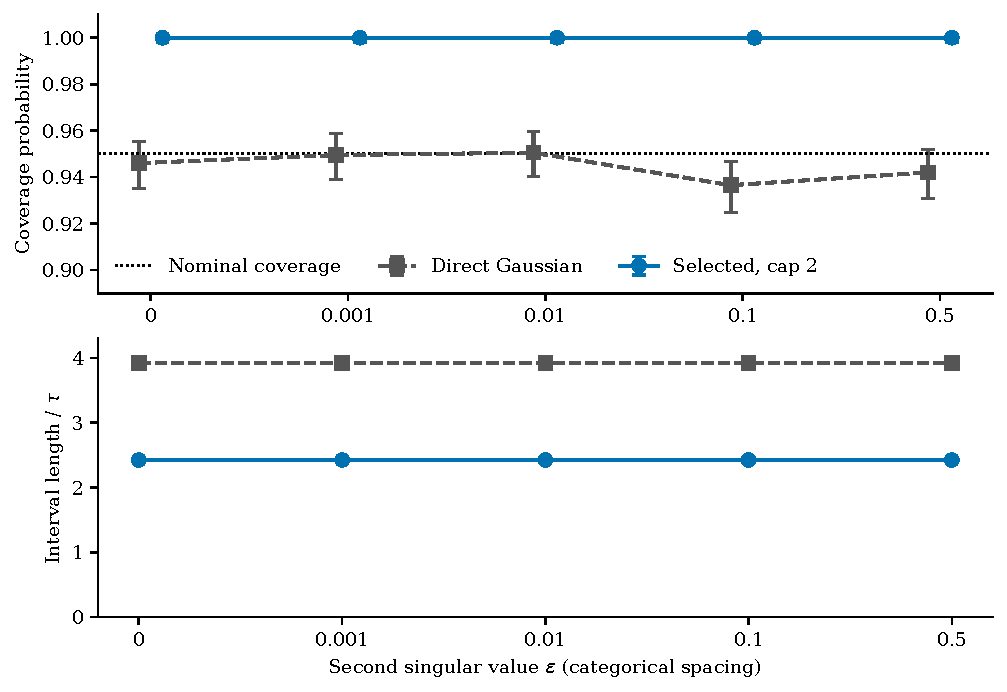
\includegraphics[width=\textwidth]{figures/weak_rank_coverage.pdf}
\caption{Coverage persists in the tested weak-component sequence, but the cap-based radius does not adapt to the actual rank. The setting is $K=3$, $p=n=8192$, $M=\sigma=1$ and cap two, with disjoint single-coordinate product factors. Top: empirical coverage and exact 95\% binomial intervals from 2,000 replications per value. Bottom: deterministic length divided by $\tau$. The horizontal spacing in $\epsilon$ is categorical.}
\label{fig:weak}
\end{figure}

Three additional zero-mean stress configurations use independent variance-one Student $t_3$ errors, a Gaussian mixture with 5\% of noise standard deviations multiplied by ten, and equicorrelated Gaussian coordinates with correlation 0.2. Table~\ref{tab:stress} reports the results. Variance contamination causes severe undercoverage for both procedures. Correlated Gaussian coordinates invalidate the direct iid variance but preserve the marginal Gaussian union bound used for the nonlinear interval. The Student result at zero is not a robustness theorem or evidence of coverage elsewhere.

\begin{table}[ht]
\centering
\begin{tabular}{lrr}
\toprule
Noise & Direct & Selected \\
\midrule
gaussian & 0.9540 & 1.0000 \\
student t3 & 0.9585 & 0.9670 \\
variance contamination & 0.5740 & 0.3830 \\
correlated & 0.1430 & 1.0000 \\
\bottomrule
\end{tabular}

\caption{Noise-assumption stress at $A=0$, $K=3$, $p=n=512$, cap one and nominal level 0.95. Only the first row belongs to the stated iid Gaussian model. These results delimit the calibration; they do not support a robustness claim.}
\label{tab:stress}
\end{table}


\subsection{Limited scan implementation}
A separate prototype implements complete support levels one and two with predetermined sphere nets. At level one the sphere is $\{-1,1\}$; at level two an equally spaced circle net with $\lceil2\pi K\rceil$ points has covering distance at most $1/(2K)$. Every product direction is evaluated, in batches. Gaussian thresholds use the actual cardinality and a simultaneous error budget.

For $K=3$, $p\in\{8,16,32\}$, $\tau=1$ and $M=\sqrt p$, we evaluated zero, one-coordinate and diffuse-support rank-one signals, with 100 replications per configuration and seed 20260912. Table~\ref{tab:scan_runtime} reports zero-signal runtimes; all nine configurations and Monte Carlo uncertainty are retained in the project. The original structural interval is selected at these dimensions: every observed length is $2\tau$ and coverage is one in the 100 replications. The corresponding exact 95\% binomial interval is approximately $[0.9638,1]$. These are implementation and cost checks, not validation of minimax projection or evidence of a finite-dimensional precision improvement.

\begin{table}[ht]
\centering\small
\begin{tabular}{rrr}
\toprule
$p$ & Product contractions & Median time (ms)\\
\midrule
8 & 192,116 & 0.197 \\
16 & 823,208 & 1.304 \\
32 & 3,402,320 & 5.737 \\
\bottomrule
\end{tabular}
\caption{Complete level-one and level-two scan costs for the prototype. Timing excludes noise generation and net preparation, uses batches and one OpenBLAS thread, and reflects the recorded macOS ARM64 environment.}\label{tab:scan_runtime}
\end{table}

\subsection{New robust and adaptive experiments}\label{sec:robust_experiments}

Four separate suites address experiments absent from the preceding report. They use fixed seeds, exact binomial confidence intervals, per-configuration source/result records and timing measurements. There are 106 configurations and 76600 Monte Carlo repetitions. Earlier experiment outputs are unchanged. The new code implements the separated SVD/projection interval, an efficient threshold-based loading correction, directional medians on a complete small product-net scan, and approximate-rank threshold intervals. It does not implement the ideal minimax residual optimizer.

\paragraph{Actual-rank calibration and precision.}
At $K=3,p=8$, the mean is a sum of zero, one, or two equal diagonal product components. Nonzero singular values are $0.25$, $3$, $100$, or $1000$ times the explicit pilot bound. Two independent observations are generated under Gaussian, Rademacher, or correlated Gaussian errors; the latter have covariance $0.5I+0.5uu^\top$ for a unit flat vector $u$. Loadings are the equal diagonal or its normalized mixture with a known off-diagonal product atom. Each of 54 configurations uses 500 repetitions. Forty-two configurations satisfy the separation condition; twelve deliberately violate it. The algorithm is supplied $M$ and noise scales but no ranks.

Over the valid configurations, minimum observed coverage is $0.944$, with exact 95\% binomial interval $[0.9201,0.9625]$, and all ranks are recovered in all repetitions. These extrema are descriptive and are not simultaneous coverage guarantees. For Gaussian equal loading at strength $1000$, rank-one and rank-two mean length/direct-length ratios are $0.480$ and $0.665$, with coverages $0.992$ and $0.988$. At strengths $3$ and $100$ the bias certificate selects the direct interval. Thus identification occurs well before useful precision improvement under this conservative certificate. All twelve below-gap configurations have zero coverage because thresholded ranks are zero although the target is not. This explicitly rejects transferring the method's coverage to weak signals.

\begin{figure}[ht]
\centering
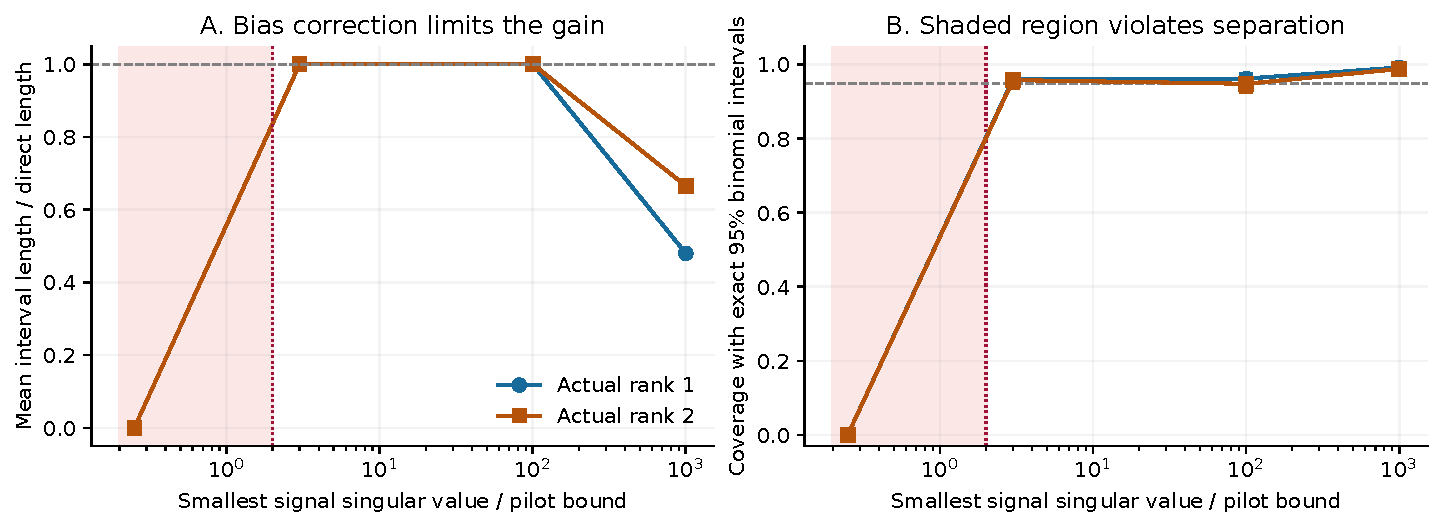
\includegraphics[width=\textwidth]{../figures/adaptive_intervals.pdf}
\caption{Implemented rank calibration under Gaussian noise and equal loading. Left: expected-length estimates relative to the direct interval. Right: coverage and exact binomial uncertainty. The shaded range violates the theorem's separation assumption. Large multiples of the conservative pilot bound represent extremely strong signals.}\label{fig:adaptive_new}
\end{figure}

\paragraph{General loading correction.}
For $K=4$, $p\in\{256,4096\}$, $M=\sqrt p$ and noise scale one, use
$L=\sqrt{1-\epsilon^2}L_{\rm flat}+\epsilon U_{\rm off}$ with
$\epsilon\in\{0,0.03,0.3\}$. The off-diagonal unit product atom is orthogonal to the flat diagonal loading. Coordinate, diffuse rank-one and off-diagonal rank-one signals, with Gaussian or independent sign errors, produce 36 configurations with 1000 repetitions each. Only the required diagonal and off-diagonal observations are generated; these have exactly the same joint law as the contractions of the full tensor. The efficient interval combines the earlier threshold center with the measured residual loading term and the required noise radius, using deterministic structural/direct fallbacks.
Coverage is at least $0.998$ on this grid. At Gaussian $p=4096$, the three remainder sizes yield lengths $0.794$, $0.928$, and $2.102$, compared with direct length $3.920$. Omitting the residual correction gives zero coverage for the off-diagonal signal at the two positive remainder sizes. These comparisons support correct calibration of the implemented upper construction, not minimax optimality for arbitrary loadings.

\paragraph{Finite-variance full scan.}
At $p=2,K=3$, all support levels are evaluated using the two singleton contractions and $19^3$ product directions on the full block, for 6861 distinct evaluated directions. A circle net with 19 points has the required covering distance. Actual direction counts are used in the block calibration, which is valid in place of a larger cardinality upper bound. There are $n=128$ independent replicates and 400 repetitions under each of Gaussian, independent signs, variance-one Student $t_3$, and variance-one rare-outlier errors. The last law is
$\sqrt{0.1}g+\sqrt{0.9/\varepsilon}\,B\xi$, with independent $g\sim N(0,1)$, $B\sim\operatorname{Bernoulli}(\varepsilon)$, sign $\xi$, and $\varepsilon=10^{-4}$, independently across entries and replicates.

The simultaneous median envelope covers in 400/400 repetitions for every law; the exact 95\% lower confidence bound is approximately $0.991$. Gaussian calibration of sample means covers in 399/400, 399/400, 390/400, and 349/400, respectively. Median thresholds are conservative. This tests the full implemented noise envelope, which is invariant to adding a mean, and does not simulate confidence-set extrema or an optimized minimax interval. Median runtime is approximately 1.6 milliseconds per repetition in the recorded single-thread environment, excluding noise generation and net construction.

\begin{figure}[ht]
\centering
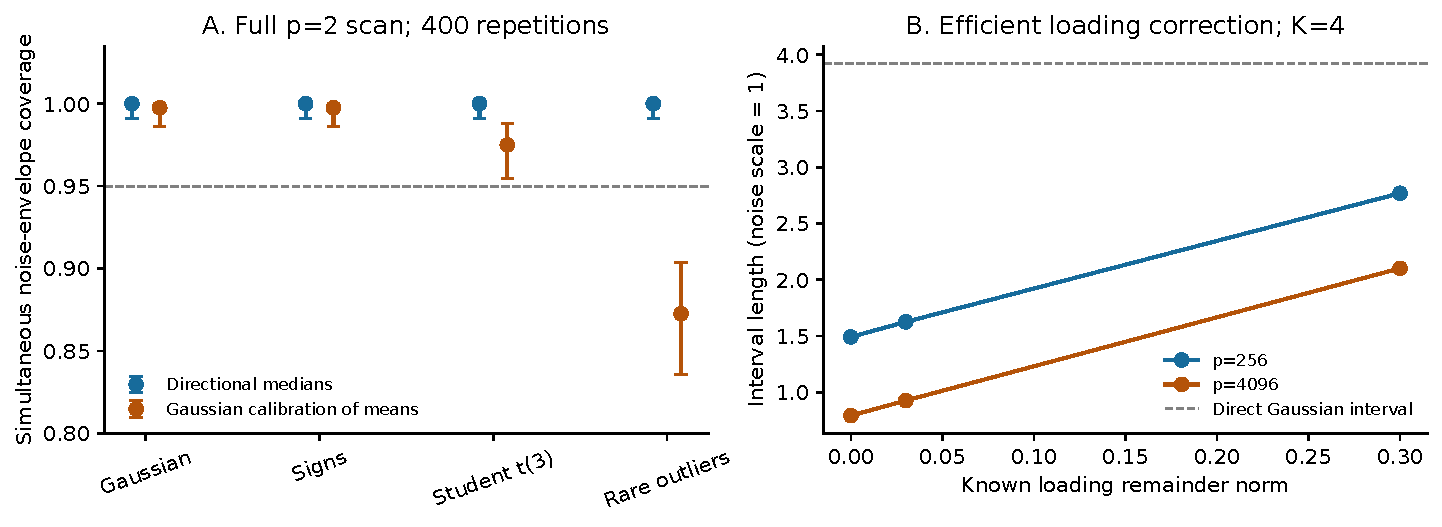
\includegraphics[width=\textwidth]{../figures/robustness_and_loadings.pdf}
\caption{Left: simultaneous full-net envelope coverage with exact binomial intervals. Gaussian mean calibration is deliberately applied outside its proxy-one assumptions for the two heavy-tailed laws. Right: lengths of the efficient corrected-loading interval under Gaussian noise.}\label{fig:robust_new}
\end{figure}

\paragraph{Approximate rank and independent checks.}
At $K=4,p=4096,M=64$, a zero, coordinate or diffuse rank-one base is perturbed by $\eta L_{\rm flat}$, with $\eta\in\{0,0.1,0.5,2\}$. Nonzero perturbations have full diagonal rank and norm $\eta$. The implemented threshold interval uses the previously proved approximation inflation, with deterministic direct/structural selection. Each configuration has 1000 repetitions; minimum observed coverage is $0.944$. At a zero base and $\eta=0.5$, inflated coverage is one and uninflated coverage is zero. At $\eta=2$ the direct interval is selected. This tests a computable valid approximate-rank procedure, not the new sharp residual projection.

Separate finite mathematical checks pass for 200 projector/bias cases, 26595 median-tail comparisons, 112086 growing-rank support pairs and 100 shifted-block constructions. They include projection self-adjointness and idempotence, the pairwise second-order bound, integration of the median excess tail, and full likelihood mixture calculations. These checks supplement proofs rather than replace them. A certified implementation of the ideal robust optimizer, a tighter moderate-signal bias certificate, and a fair implementation comparison under a common regular-signal model remain outstanding.


\section{Discussion}\label{sec:discussion}

The results show that the parameter class over which coverage is required can determine the order of an honest interval's length. For a prescribed orthogonal contrast, simultaneous tensor rank restrictions yield an interval smaller than the order required by a single-unfolding relaxation. The comparison holds at arbitrarily weak signals and does not depend on identifying the actual rank. It also separates nonlinear procedures from every fixed-radius affine interval on the original class.

The exact diagonal reduction gives a precise connection with classical sequence inference. At rank one, the attainable diagonal vectors form an $\ell_{2/K}$ ball; Proposition~\ref{prop:diagonal_minimax} then identifies the optimal rate among diagonal-based intervals. The residual confidence-set projection and sparse harmonic mixture quantify the value of off-diagonal observations. At $M=\tau\sqrt p$, both $\mathcal L_0$ and $\mathcal L_{\max}$ have rate $\tau(\log p)^{3/2}/\sqrt p$ for $K=3$, and $\tau\sqrt{\log p/p}$ for fixed $K\ge4$. These are statistical minimax statements; the exact projection may be computationally expensive. Similarly, Theorem~\ref{thm:unfolding} applies to a larger honesty class, not to every algorithm that represents its data as a matrix.

Several restrictions affect practical inference. The loading must have the orthogonal product form, the Frobenius and rank caps are supplied, and the noise standard deviation is known. Appendix~\ref{app:refinements} improves the cap coefficient and relaxes the noise and exact-rank assumptions under explicit calibration. These refinements do not provide automatic adaptation when a singular value vanishes. The experiments show substantial conservatism even though length improves over the specified benchmarks. Strong-signal subspace inference or a known-direction oracle may give better pointwise precision.

Theorem~\ref{thm:all_norm_rates} removes the original norm/noise scaling restriction, and Theorem~\ref{thm:all_norm_mse} supplies squared-risk control even for arbitrarily large $M/\tau$. Theorem~\ref{thm:weighted_bounds} gives nonuniform orthogonal loading bounds, while Proposition~\ref{prop:flat_loading} identifies sharp support-size dependence. These loading bounds need not match for arbitrary unequal weights. The remaining computational question is whether an efficient procedure can attain the full-data minimax interval rate. The truncated scan gives an explicit search budget, while Theorem~\ref{thm:low_degree} rules out minimax squared-error estimation by a range of polynomial degrees. This restricted result cannot be promoted to a lower bound against all polynomial-time interval procedures. Sharp general loading geometry and actual-rank adaptation remain further questions: they require a characterization of which contrasts benefit from joint constraints and which smaller-rank subclasses can be distinguished while retaining outer-class honesty.

Section~\ref{sec:robust_adaptive} supplies positive results with precise boundaries. Full-data upper rates require directional concentration, not Gaussianity; finite-variance replicate rates use calibrated directional medians and sufficient replication. Minimax lower bounds over those unknown-law families follow from their Gaussian subfamilies, not from a universal equivalence of noise laws. Approximate ranks admit a sharp additive allowance for interval length. The separated SVD/projection construction is computable for arbitrary loadings and selects actual mode ranks, but its bias certificate can require very strong signals before length improves. Its coverage is not asserted on the original unseparated class. A convex outer-class obstruction limits full convexification, while the shifted-mixture bound extends the adaptation obstruction beyond zero. None of these statements supplies an efficient minimax interval in the original difficult regime.

Applications require a sampling model that justifies the noise calibration and an independently specified contrast. Repeated calibrated tensor measurements could provide such a model, but no real-data experiment is claimed here. In particular, arrays indexed by LLM model, layer and prompt generally have prompt, token and layer dependence, heterogeneous noise and data-derived loadings. Simply stacking those observations does not establish the Gaussian experiment. The noise-envelope extension in Appendix~\ref{app:refinements} is one ingredient, but a justified dependence model and functional-selection theory would still be necessary before an LLM experiment could substantiate these inferential claims.

\paragraph{Reproducibility.}
The accompanying project contains the simulation protocol, modular Python code, fixed seeds, 817 result rows, exact binomial uncertainty, source and result hashes, the literature matrix and a theorem-status ledger. The original simulation outputs are reused without changing the interval algorithm. The theory review adds exact finite checks of the new sign-mixture calculation, approximation inequalities and affine bounds. The earlier review did not simulate the exhaustive scan. The subsequent development includes exact sparse-mixture and Hermite-moment checks and a finite-net prototype. All displayed numerical values come from saved outputs or analytic formulas. The norm/loading extension adds separate finite checks of the uniform-rate envelopes, weighted full-tensor mixtures, residual-noise tails, and orthogonal embeddings; these are not simulations of the ideal residual optimizer.

\appendix
\section{Complete proofs}\label{app:proofs}

The proofs apply in finite dimensions. Constants used in the main text are explicit. All tensors and Gaussian variables are real.

\subsection{Canonical product expansions}

\begin{lemma}[Controlled squared component weights]\label{lem:cp}
For a tensor in either cap class there is a finite representation
\[
 A=\sum_{j=1}^{J_A}x_{1j}\otimes\cdots\otimes x_{Kj},\qquad
 a_j^{\mathrm{cp}}=\prod_{k=1}^K\norm{x_{kj}}_2,
\]
such that $J_A\le J$ and $\sum_j(a_j^{\mathrm{cp}})^2=\norm A_F^2$.
\end{lemma}


\noindent\emph{Roadmap.} Choose orthonormal Tucker mode bases or left-orthogonal TT cores; expand product terms and sum their squared weights. The TT argument uses a prefix identity, not orthogonality of individual paths.
\begin{proof}
The zero tensor has a zero-term representation. For a nonzero Tucker tensor, choose orthonormal bases $U_k$ for the column spaces of its mode unfoldings. Orthogonal projection onto each such space leaves $A$ unchanged. Contracting these bases gives a core $\mathcal G$ with $A=\mathcal G\times_1U_1\cdots\times_KU_K$ and $\norm{\mathcal G}_F=\norm A_F$. The actual mode ranks satisfy $r_k\le\bar r_k$.

Fix a mode $k$. Expand all core indices other than $k$. Each tuple $j_{-k}$ gives unit factors $U_\ell[:,j_\ell]$ in modes $\ell\ne k$ and factor $U_k\mathcal G[:,j_{-k}]$ in mode $k$. Its squared product weight is $\norm{\mathcal G[:,j_{-k}]}_2^2$. These slice squares sum to $\norm{\mathcal G}_F^2$. The number of terms is $\prod_{\ell\ne k}r_\ell$. Choosing $k$ to minimize the corresponding cap product proves the Tucker assertion.

For a TT tensor, sequential matrix factorizations yield cores $G_k\in\R^{r_{k-1}\times p_k\times r_k}$, with $r_0=r_K=1$ and $r_k\le\bar r_k$. At each cut, factor the relevant matrix through a basis of its column space. Equivalently, left-orthogonalize the cores by QR and absorb the triangular factors into the next core. Thus the $(r_{k-1}p_k)\times r_k$ matrix associated with $G_k$ has orthonormal columns for $k<K$, and $\norm{G_K}_F=\norm A_F$. These steps use no inverse lower bound on a singular value.

Expand the contraction over all internal paths $(a_1,\ldots,a_{K-1})$. A path contributes the product tensor with physical vectors $G_k[a_{k-1},:,a_k]$. There are at most $\prod_{k<K}r_k\le J$ paths. To sum their squared weights, let
\[
 t_k(b)=\sum_{a_1,\ldots,a_{k-1}}
 \prod_{\ell=1}^k\norm{G_\ell[a_{\ell-1},:,a_\ell]}_2^2,
 \qquad a_k=b.
\]
Column normalization gives $t_1(b)=1$. If $t_{k-1}(a)=1$ for all $a$, then
\[
 t_k(b)=\sum_a t_{k-1}(a)\norm{G_k[a,:,b]}_2^2=1
\]
for $k<K$. Hence the sum of all squared path weights is
\[
 \sum_a t_{K-1}(a)\norm{G_K[a,:,1]}_2^2=\norm{G_K}_F^2=\norm A_F^2.
\]
The individual path terms need not be orthogonal; the prefix identity is what proves the required equality.
\end{proof}

\subsection{Proof of Theorem~\ref{thm:diagonal}}


\noindent\emph{Roadmap.} Apply subadditivity, modewise H\"older and Bessel, then control the component-weight sum.
\begin{proof}
Let $q=2/K\le1$ and use Lemma~\ref{lem:cp}. Subadditivity of the $q$th power of absolute value gives
\[
 \sum_i|\ip A{V_i}|^q
 \le\sum_j\sum_i\prod_{k=1}^K|\ip{x_{kj}}{v_{ki}}|^{2/K}.
\]
H\"older's inequality with $K$ equal exponents, followed by Bessel's inequality for each orthonormal family, yields
\begin{align*}
 \sum_i\prod_k|\ip{x_{kj}}{v_{ki}}|^{2/K}
 &\le\prod_k\left(\sum_i|\ip{x_{kj}}{v_{ki}}|^2\right)^{1/K}\\
 &\le\prod_k\norm{x_{kj}}_2^{2/K}=(a_j^{\mathrm{cp}})^q.
\end{align*}
Finally, the power-mean inequality (or H\"older with exponents $2/q$ and $2/(2-q)$) gives
\[
 \sum_j(a_j^{\mathrm{cp}})^q
 \le J_A^{1-q/2}\left\{\sum_j(a_j^{\mathrm{cp}})^2\right\}^{q/2}
 \le J^{1-q/2}M^q.
\]
This is \eqref{eq:compress}. For $J_A=0$ both sides of the first inequality are zero.
\end{proof}

\subsection{Exact rank-one diagonal image}

\begin{lemma}[Exact diagonal reduction]\label{lem:image}
Under \eqref{eq:loading}, the image of the rank-one tensor Frobenius ball of radius $M$ under $A\mapsto(\ip A{V_i})_{i=1}^m$ is exactly
\[
 \left\{a\in\R^m:\sum_i|a_i|^{2/K}\le M^{2/K}\right\}.
\]
\end{lemma}


\noindent\emph{Roadmap.} Use the diagonal bound for one inclusion and construct signed product factors for the converse.
\begin{proof}
One inclusion follows from Theorem~\ref{thm:diagonal} with $J=1$. Conversely, for any vector in the displayed ball, put
\[
 x_1=\sum_i\operatorname{sign}(a_i)|a_i|^{1/K}v_{1i},\qquad
 x_k=\sum_i|a_i|^{1/K}v_{ki},\quad k\ge2,
\]
and set $A=x_1\otimes\cdots\otimes x_K$. Orthonormality gives $\ip A{V_i}=a_i$ and
\[
 \norm A_F=\prod_k\norm{x_k}_2
 =\left(\sum_i|a_i|^{2/K}\right)^{K/2}\le M.
\]
The tensor has every Tucker and TT rank at most one. The zero vector is handled by the zero tensor.
\end{proof}

\subsection{Threshold error and structural radius}

\begin{lemma}[Scalar threshold envelope]\label{lem:soft}
If $|e|\le\lambda$ and $s=\soft_\lambda(x+e)$, then $s$ lies between zero and $x$ and
\[
 |s-x|\le\min(|x|,2\lambda).
\]
For $q\in(0,1]$, $t,u\ge0$, one also has $\min(t,u)\le t^q u^{1-q}$, with the continuous interpretation at zero.
\end{lemma}


\noindent\emph{Roadmap.} Check positive and negative scalar inputs, then interpolate the two deterministic error bounds.
\begin{proof}
For $x\ge0$, $x+e\ge-\lambda$, so thresholding cannot produce a negative value. Also $x+e-\lambda\le x$, so $0\le s\le x$. If $x>2\lambda$, then $x+e>\lambda$ and $x-s=\lambda-e\le2\lambda$. Otherwise $x-s\le x\le2\lambda$. The negative case follows by oddness. If $t\le u$, then $t=t^q t^{1-q}\le t^q u^{1-q}$; if $u\le t$, then $u=u^q u^{1-q}\le t^q u^{1-q}$.
\end{proof}

\begin{lemma}[Matrix functional bound]\label{lem:structural}
If $\rank(B)\le r$ and $H$ has singular values $s_1(H)\ge s_2(H)\ge\cdots$, then
\[
 |\ip HB|\le\norm B_F\left(\sum_{i\le r}s_i(H)^2\right)^{1/2}.
\]
\end{lemma}


\noindent\emph{Roadmap.} Project onto the matrix column space and maximize the spectral trace over projections of bounded rank.
\begin{proof}
Let $P$ project onto the column space of $B$. Then $PB=B$ and Cauchy--Schwarz gives $|\ip HB|=|\ip{PH}B|\le\norm{PH}_F\norm B_F$. Write $HH^\top=\sum_i\lambda_i u_i u_i^\top$, with decreasing nonnegative eigenvalues. The numbers $b_i=u_i^\top P u_i$ satisfy $0\le b_i\le1$ and $\sum_i b_i=\operatorname{tr}(P)\le r$. Therefore $\norm{PH}_F^2=\sum_i\lambda_i b_i\le\sum_{i\le r}\lambda_i$: moving any weight from a smaller eigenvalue to an unfilled larger one cannot reduce this sum. Since $\lambda_i=s_i(H)^2$, the result follows.
\end{proof}

\subsection{Proof of Theorem~\ref{thm:coverage}}


\noindent\emph{Roadmap.} Construct a uniform coordinate-noise event, bound the threshold error pathwise, verify the other intervals and use the deterministic selection rule.
\begin{proof}
The product atoms are orthonormal because
\[
 \ip{V_i}{V_j}=\prod_k\ip{v_{ki}}{v_{kj}}=\mathbf1\{i=j\}.
\]
Gaussian isotropy then gives the independent normals in \eqref{eq:diagonal}. For a standard normal $g$, Chernoff's inequality gives $\PP(g>t)\le\exp(-t^2/2)$ by minimizing $\exp(-ut+u^2/2)$ at $u=t$. Apply the same inequality to $-g$ and take a union bound to obtain
\[
 \PP\{\max_i|\tau g_i|>\lambda\}
 \le2m\exp\{-\lambda^2/(2\tau^2)\}=\alpha.
\]
On the complementary event, Lemma~\ref{lem:soft} and Theorem~\ref{thm:diagonal} give
\begin{align*}
 |\widehat\psi_{\NL}-\psi(A)|
 &\le\norm w_\infty\sum_i\min(|a_i|,2\lambda)\\
 &\le\norm w_\infty(2\lambda)^{1-q}\sum_i|a_i|^q\le h_{\NL}.
\end{align*}
This proves the uniform coverage of $I_{\NL}$.

Because $\norm L_F=1$, $\ip LZ-\psi(A)\sim N(0,\tau^2)$, so $I_G$ has exact coverage. For any constrained unfolding, the loading matrix has singular values $|w_i|$: the product vectors on each side form orthonormal families. Lemma~\ref{lem:structural} thus gives $|\psi(A)|\le M(\sum_{i\le r}w_{(i)}^2)^{1/2}$. Choosing the smallest cap proves $|\psi(A)|\le h_0$, so $I_0$ has coverage one. The selected index in \eqref{eq:select} is deterministic, hence the selected interval retains its individual coverage without a multiple-selection correction. Its length is exactly \eqref{eq:length}.
\end{proof}

\subsection{Proof of Theorem~\ref{thm:affine}}


\noindent\emph{Roadmap.} Force a variance cost at zero and a bias cost at signed coordinate tensors, then combine the two necessary inequalities.
\begin{proof}
Set $t=\ip WL$. At $A=0$ the center error is normal with mean $b$ and standard deviation $v=\tau\norm W_F$. For fixed $h$ and $v>0$, the probability that this variable belongs to $[-h,h]$ is maximized at $b=0$. Indeed, for $b\ge0$ its derivative is
\[
 v^{-1}\{\phi((h+b)/v)-\phi((h-b)/v)\}\le0,
\]
since $|h+b|\ge|h-b|$; the function is even in $b$. Honesty at zero therefore implies $h\ge z\tau\norm W_F\ge z\tau|t|$. If $v=0$, the same last inequality is automatic.

At $A=\pm M E_i$, the mean center error is
\[
 b\pm M(\ip W{E_i}-p^{-1/2}).
\]
At least one sign has absolute mean at least $M|\ip W{E_i}-p^{-1/2}|$. A symmetric interval whose radius is strictly smaller than this mean magnitude has probability below $1/2$ under a nondegenerate normal distribution: it lies strictly to one side of the median. In the degenerate case the coverage is zero. Since $1-\alpha>1/2$, honesty forces
\[
 h\ge M\max_i|\ip W{E_i}-p^{-1/2}|
 \ge\frac M{\sqrt p}|1-t|.
\]
The last inequality follows from $t-1=p^{-1/2}\sum_i(\ip W{E_i}-p^{-1/2})$. Put $a=M/\sqrt p$ and $b'=z\tau$. The two bounds imply
\[
 1\le|1-t|+|t|\le h/a+h/b',
\]
which rearranges to \eqref{eq:affinelower}. On the rank-one tensor ball, $h_0=M/\sqrt p$, and the direct/structural choice gives the matching order. No result about arbitrary data-dependent widths is invoked.
\end{proof}

\subsection{A mixture inequality for confidence intervals}

\begin{lemma}[Common-target alternatives]\label{lem:mixture}
Let $P_0$ have target zero and let $Q$ be a mixture of alternatives whose targets all equal $\delta>0$. If $C$ covers zero under $P_0$ and covers the target at every alternative with probability at least $1-\alpha$, then
\begin{equation}\label{eq:mixtureCI}
 \E_0|C|\ge\delta\{1-2\alpha-\TV(P_0,Q)\}.
\end{equation}
If $Q\ll P_0$, then $\TV(P_0,Q)\le\frac12\sqrt{\chi^2(Q,P_0)}$.
\end{lemma}


\noindent\emph{Roadmap.} Transfer coverage from the common-target mixture to the null using total variation, then intersect the two coverage events.
\begin{proof}
Mixture coverage gives $Q(\delta\in C)\ge1-\alpha$. By the definition of total variation, $P_0(\delta\in C)\ge1-\alpha-\TV(P_0,Q)$. Intersecting with $\{0\in C\}$ gives probability at least $1-2\alpha-\TV$. An interval containing both points has length at least $\delta$, proving \eqref{eq:mixtureCI}. The divergence bound follows from Cauchy--Schwarz applied to $\frac12\E_0|dQ/dP_0-1|$. Appending an independent random seed leaves total variation unchanged, so randomized intervals are covered as well.
\end{proof}

For Gaussian shifts $P_B=N(\operatorname{vec}(B),\tau^2I_D)$, direct integration of their likelihood ratios gives
\begin{equation}\label{eq:LR}
 \E_0\left[\frac{dP_B}{dP_0}\frac{dP_C}{dP_0}\right]
 =\exp\{\ip BC/\tau^2\}.
\end{equation}
To verify this, each ratio is $\exp\{\ip ZB/\tau^2-\norm B_F^2/(2\tau^2)\}$. Multiply the ratios and use the moment generating function of $\ip Z{B+C}$, whose variance under $P_0$ is $\tau^2\norm{B+C}_F^2$. The exponent simplifies to \eqref{eq:LR}.

\subsection{Proof of Theorem~\ref{thm:unfolding}}


\noindent\emph{Roadmap.} Construct rank-one matrix alternatives within the chosen unfolding and bound their full Gaussian likelihood second moment using an auxiliary Gaussian.
\begin{proof}
For the given bipartition, let $f_i=\bigotimes_{k\in S}e_i$ and $g_i=\bigotimes_{k\notin S}e_i$. Both families are orthonormal. Let $u=p^{-1/2}(s_1,\ldots,s_p)$ with independent uniform signs, and define
\[
 \theta=\min(M,\tau\sqrt p/4),\qquad
 A_u=\theta\left(\sum_i u_i f_i\right)\otimes
                    \left(\sum_j u_j g_j\right).
\]
Every alternative has rank one in this unfolding, norm $\theta$, and functional value $\delta=\theta/\sqrt p$. Let $Q$ average their Gaussian laws. If $v$ is an independent copy of $u$, then \eqref{eq:LR} gives
\[
 1+\chi^2(Q,P_0)=\E_{u,v}\exp\{\theta^2(u^\top v)^2/\tau^2\}
 =\E\exp\{a S_p^2/p\},
\]
where $S_p$ is a sum of $p$ independent signs and $a=\theta^2/(\tau^2p)\le1/16$.

Introduce an independent standard normal $H$. Its moment generating function yields
\begin{align*}
 \E\exp(aS_p^2/p)
 &=\E_H\left\{\cosh(\sqrt{2a/p}\,H)\right\}^p\\
 &\le\E_H\exp(aH^2)=(1-2a)^{-1/2}\le\sqrt{8/7}.
\end{align*}
The inequality uses $\log\cosh(x)\le x^2/2$: for $x\ge0$, its derivative $\tanh(x)$ is at most $x$, and both functions are even. The Gaussian-square expectation follows by integrating $\exp\{-(1-2a)h^2/2\}/\sqrt{2\pi}$; it is finite since $a<1/2$. Nonnegative integrands justify exchanging the expectations.

Lemma~\ref{lem:mixture} now gives \eqref{eq:unfoldlower}. The constant is positive for $\alpha<1/4$. On $\Theta_S$, Lemma~\ref{lem:structural} with loading singular values all equal to $p^{-1/2}$ gives $|\psi(A)|\le M/\sqrt p$. Choosing between this structural interval and the direct interval attains the lower order. All calculations use the entire Gaussian experiment; the result does not arise from hiding off-diagonal observations.
\end{proof}

\subsection{Proof of Theorem~\ref{thm:separation}}


\noindent\emph{Roadmap.} Substitute the specified dimensions and norm scaling, then apply the two lower-bound theorems with their confidence-level restrictions.
\begin{proof}
Substitute $M=\tau\sqrt p$, $q=2/K$ and $\norm w_\infty=p^{-1/2}$ into \eqref{eq:nl}. This gives
\[
 h_{\NL}=\tau J^{1-1/K}
 p^{1/K-1/2}\{8\log(2p/\alpha)\}^{(K-2)/(2K)},
\]
which is the radius in \eqref{eq:separation}. For fixed $K\ge3$, its exponent $\beta=(K-2)/(2K)$ is positive and $(\log p/p)^\beta\to0$. The cap classes contain all $\pm M E_i$ and zero, so Theorem~\ref{thm:affine} gives radius at least $z\tau/(1+z)$. For any retained constrained unfolding, the corresponding matrix-rank cap class contains $\Theta_S$, and Theorem~\ref{thm:unfolding} gives expected length at zero at least $c_\alpha\tau/4$. The same comparisons under the stated growing-cap condition follow by retaining the factor $J^{1-1/K}$.
\end{proof}

\subsection{Proof of Theorem~\ref{thm:jointlower}}


\noindent\emph{Roadmap.} Mix orthogonal coordinate shifts, compute the full likelihood second moment exactly and apply the interval mixture lemma.
\begin{proof}
Let $a=\min\{M,\tau\sqrt{\log(1+p/4)}\}$ and mix uniformly over $A_j=aE_j$, $j=1,\ldots,p$. Each is in the rank-one tensor class and has target $\delta=a/\sqrt p$. Orthogonality of the $E_j$ and \eqref{eq:LR} imply
\[
 1+\chi^2(Q,P_0)=p^{-2}\{p\exp(a^2/\tau^2)+p(p-1)\}.
\]
Thus $\chi^2(Q,P_0)=\{\exp(a^2/\tau^2)-1\}/p\le1/4$ and $\TV(P_0,Q)\le1/4$. Lemma~\ref{lem:mixture} gives \eqref{eq:jointlower}. This construction does not establish that these alternatives are least favorable.
\end{proof}


\subsection{Proof of Proposition~\ref{prop:diagonal_minimax}}


\noindent\emph{Roadmap.} Construct sparse diagonals inside the rank-one tensor class, bound the diagonal likelihood mixture using factorial moments and balance the support size. The full-data likelihood is kept separate.
\begin{proof}
For an integer $1\le s\le p$, let $S$ be a uniformly chosen size-$s$ subset of $\{1,\ldots,p\}$. Define
\[
 A_S=b_s\left(\sum_{i\in S}e_i\right)^{\otimes K}.
\]
This is a rank-one tensor, $\norm{A_S}_F=b_s s^{K/2}\le M$, and every alternative has target $\delta_s=s b_s/\sqrt p$. Its observed diagonal has mean $b_s\mathbf1_S$. Let $Q_d$ be the uniform mixture of these diagonal Gaussian laws, and let $P_{0,d}$ be the zero-mean diagonal law. Applying the Gaussian shift calculation \eqref{eq:LR} in dimension $p$ gives
\begin{equation}\label{eq:diag_chisquare}
 1+\chi^2(Q_d,P_{0,d})
 =\E_{S,T}\exp\{b_s^2|S\cap T|/\tau^2\},
\end{equation}
where $S,T$ are independent uniform size-$s$ subsets. This is the sparse-mixture mechanism used in classical sequence lower bounds \citep{collier2017}; the following counting argument records the needed bound explicitly.

Conditional on $S$, $H=|S\cap T|$ is hypergeometric with population size $p$, success count $s$ and sample size $s$. Write $(x)_j=x(x-1)\cdots(x-j+1)$, with $(x)_0=1$. Counting the $j$-element subsets of $S$ contained in $T$ yields
\[
 \E\binom Hj=\binom sj\frac{(s)_j}{(p)_j}
 \le\binom sj(s/p)^j,\qquad 0\le j\le s.
\]
For $j\ge1$, the inequality follows factor by factor from
$(s-\ell)/(p-\ell)\le s/p$ for $0\le\ell<j$, since $s\le p$.
Set $t=\exp(b_s^2/\tau^2)-1\ge0$. Expanding $(1+t)^H$ and using the preceding factorial moments gives
\begin{align*}
 \E\exp(b_s^2H/\tau^2)
 &=\sum_{j=0}^s t^j\E\binom Hj\\
 &\le (1+st/p)^s
 \le \exp(s^2t/p)
 \le e^{1/4}.
\end{align*}
The last inequality uses the definition of $b_s$. Equation~\eqref{eq:diag_chisquare} and Cauchy--Schwarz therefore give
\[
 \TV(Q_d,P_{0,d})\le\frac12\sqrt{e^{1/4}-1}.
\]
Lemma~\ref{lem:mixture}, now applied to the diagonal experiment, proves \eqref{eq:diagonal_lower}. The constant is positive because $\alpha<1/4$ and $\frac12\sqrt{e^{1/4}-1}<1/2$. The argument also covers independent randomization.

To prove \eqref{eq:diagonal_rate}, let
$x_p=(p/\log p)^{1/K}$ and $s_p=\lfloor x_p\rfloor$. For sufficiently large $p$,
$x_p/2\le s_p\le x_p$ and $s_p\ge1$. When $M=\tau\sqrt p$, the norm term in $b_{s_p}$ is at least $\tau\sqrt{\log p}$. The noise term is at most this quantity, since $1+p/(4s_p^2)\le1+p/4\le p$ for $p\ge2$. Thus the minimum equals the noise term. Since $K>2$ and $s_p\le p^{1/K}$ eventually,
\[
 \log\{1+p/(4s_p^2)\}
 \ge\log\{1+p^{1-2/K}/4\}
 \ge\tfrac12(1-2/K)\log p
\]
for sufficiently large $p$. Consequently,
\[
 \frac{s_p b_{s_p}}{\sqrt p}
 \ge \frac12\sqrt{\frac{1-2/K}{2}}\,
 \tau\left(\frac{\log p}{p}\right)^{(K-2)/(2K)}.
\]
Theorem~\ref{thm:coverage} with $J=1$ gives an upper bound of the same order and deterministic length. Since the worst-case criterion is at least the criterion at zero, both rates follow. The fixed-cap extension follows by class inclusion for the lower bound and a constant $J^{1-1/K}$ for the upper bound.

For completeness, the corresponding \emph{full-tensor} mixture would have
$\ip{A_S}{A_T}=b_s^2|S\cap T|^K$ in \eqref{eq:LR}. Its likelihood second moment is not \eqref{eq:diag_chisquare}, and the preceding bound does not apply to it. The proposition is restricted to diagonal observations throughout.
\end{proof}


\section{Proofs of the full-data refinements}\label{app:full_data_proofs}

\begin{lemma}[Finite product nets and injective norm]\label{lem:net_scan}
The nets used in \eqref{eq:scan_threshold} exist and satisfy
$\rho(B)\le2N_S(B)$ for any tensor on $S^K$.
Furthermore, a tensor $B$ in either rank-cap class satisfies
$\norm B_F\le\sqrt J\,\rho(B)$.
\end{lemma}
\noindent\emph{Roadmap.} Use a volume bound and product telescoping, then apply the canonical squared-weight identity.
\begin{proof}
A maximal $\varepsilon$-separated subset of the unit sphere is an $\varepsilon$-net. Balls of radius $\varepsilon/2$ around its points are disjoint and contained in the ball of radius $1+\varepsilon/2$. The ratio of their Euclidean volumes bounds the cardinality by $(1+2/\varepsilon)^s$. Compactness gives a finite maximal set. Take $\varepsilon=1/(2K)$.

Approximate each factor of any unit product direction by a net point. Telescoping the product one factor at a time, each contraction difference has magnitude at most $\varepsilon\rho(B)$, by multilinearity and the definition of $\rho$. The sum is at most $K\varepsilon\rho(B)=\rho(B)/2$. Taking the supremum gives $\rho(B)\le N_S(B)+\rho(B)/2$.

For the second assertion use Lemma~\ref{lem:cp}, writing its product terms as $X_j$. Then
\[
 \norm B_F^2
 =\sum_j\ip B{X_j}
 \le\rho(B)\sum_j\norm{X_j}_F
 \le\rho(B)\sqrt J
       \left(\sum_j\norm{X_j}_F^2\right)^{1/2}
 =\rho(B)\sqrt J\,\norm B_F.
\]
The middle inequality is Cauchy--Schwarz, and the last identity is the squared-weight conclusion of Lemma~\ref{lem:cp}. Divide when $B\ne0$; the zero case is immediate.
\end{proof}

\subsection{Proof of Theorem~\ref{thm:scan}}
\noindent\emph{Roadmap.} A finite Gaussian union bound controls every net contraction. Test acceptance on that event bounds each ordered diagonal coordinate. Summation gives the interval and intersection gives the two expected-length guarantees.
\begin{proof}
There are at most $(ep/s)^s$ subsets of size $s$, since
$\binom ps\le p^s/s!$ and
$\log(s!)\ge\int_1^s\log x\,dx\ge s\log s-s$.
Each unit product contraction of $\tau G$ has distribution $N(0,\tau^2)$. Therefore the Gaussian Chernoff bound gives
\begin{align*}
 \PP\{\exists S:N_S(\tau G)>\lambda_{|S|}^{\rm scan}\}
 &\le\sum_{s=1}^p
 2(ep/s)^s(1+4K)^{Ks}
     \exp\{-(\lambda_s^{\rm scan})^2/(2\tau^2)\}\\
 &\le\gamma.
\end{align*}
Let $\mathcal E_\gamma$ be the complementary event. No independence between the scanned contractions is required.

On $\mathcal E_\gamma$, if the test accepts, the triangle inequality for the finite maximum implies $N_S(A)\le2\lambda_s^{\rm scan}$. Lemma~\ref{lem:net_scan} gives $\rho(A_{S,\ldots,S})\le4\lambda_s^{\rm scan}$. Coordinate restriction cannot increase any constrained unfolding rank, because it multiplies an unfolding by selection matrices. Theorem~\ref{thm:diagonal} and Lemma~\ref{lem:net_scan} thus imply
\[
 \sum_{i\in S}|A_{i,\ldots,i}|^q
 \le J^{1-q/2}\norm{A_{S,\ldots,S}}_F^q
 \le J\,\rho(A_{S,\ldots,S})^q.
\]
Let $|a|_{(s)}$ be the $s$th largest absolute diagonal entry. Choose $S$ to contain the $s$ largest entries. It follows that
\[
 s|a|_{(s)}^q\le J(4\lambda_s^{\rm scan})^q,
 \qquad
 |a|_{(s)}\le4J^{K/2}\lambda_s^{\rm scan}s^{-K/2}.
\]
Summing these inequalities and using
$|\psi(A)|\le p^{-1/2}\sum_i|a_i|$
proves the bound $|\psi(A)|\le R_\gamma$ in \eqref{eq:scan_radius}. On rejection the structural interval covers surely. Therefore $C_{\rm scan}$ covers on $\mathcal E_\gamma$ and is honest at level $1-\gamma$.

Both intersected intervals cover with probability at least $1-\alpha_0-\gamma$. On that event the intersection is nonempty and covers; replacing empty intersections by $\{0\}$ preserves this argument. Its length is always at most $\ell_*$. At zero, the rejection probability is at most $\gamma$, and on acceptance the intersection has length at most $2R_\gamma$. This gives \eqref{eq:scan_expectation}, without independence between the intervals.

For the specified $\gamma$, elementary logarithm bounds give
$\lambda_s^{\rm scan}\le C_K\tau\sqrt{s\log(2p/\alpha)}$.
For example, use $s\log(ep/s)\le s(1+\log p)$,
$\log(2p/\gamma)\le2\log(2p/\alpha)$ and $s\ge1$.
Equation~\eqref{eq:scan_radius} now proves \eqref{eq:scan_rate}; the extra term $\ell_*\gamma$ is smaller in order by Theorem~\ref{thm:separation}.
If $K\ge4$, the sum is at most $1+2/(K-3)$ by integration of $x^{-(K-1)/2}$ over $[1,\infty)$. If $K=3$, it is at most $1+\log p$. Combining the upper bound for $K\ge4$ with Theorem~\ref{thm:jointlower} proves \eqref{eq:zero_sharp}.
\end{proof}

\begin{lemma}[Uniform cubic moment for a weighted sign sum]\label{lem:cubic_moment}
For independent uniform signs $\epsilon_i$, let
$S_p=\sum_{i=1}^p i^{-2/3}\epsilon_i$. Then, uniformly in $p\ge1$,
\[
 \PP(|S_p|>x)\le2e^{-x^3/192}\quad(x\ge12),
 \qquad
 \E\exp\{|S_p|^3/40000\}\le20/19+1/100<5/4.
\]
\end{lemma}
\noindent\emph{Roadmap.} Split the weighted sign sum into a bounded head and a sub-Gaussian tail, then integrate its cubic tail probability.
\begin{proof}
For $x\ge12$, put $m=\lfloor(x/6)^3\rfloor$. If $m\ge p$, then
$|S_p|\le3p^{1/3}\le x/2$.
Otherwise, the first $m$ terms have absolute sum at most
$3m^{1/3}\le x/2$. The remaining independent sign sum has variance proxy
\[
 V_m=\sum_{i>m}i^{-4/3}\le3m^{-1/3}\le24/x.
\]
Here $m\ge(x/6)^3/2$ and $18\cdot2^{1/3}<24$.
The product inequality $\prod_i\cosh(ti^{-2/3})\le\exp(t^2V_m/2)$
and Chernoff optimization give a two-sided tail bound
$2\exp\{-(x/2)^2/(2V_m)\}\le2e^{-x^3/192}$.

Put $u=1/40000$ and $Y=|S_p|^3$. Tonelli's theorem applied to
$e^{uY}=1+\int_0^Y ue^{ut}\,dt$ yields
\[
 \E e^{uY}
 \le e^{1728u}
 +\frac{2u}{1/192-u}
       e^{-(1/192-u)1728}
 \le \frac{20}{19}+\frac1{100}.
\]
The last step uses $1728u<1/20$, $e^x\le(1-x)^{-1}$ for $0\le x<1$,
and $1/192-u\ge1/200$. The exponential factor in the second term is at most one. These estimates are uniform in $p$.
\end{proof}

\subsection{Proof of Theorem~\ref{thm:harmonic}}
\noindent\emph{Roadmap.} Couple three rank-one factor signs so that the diagonal is deterministic and harmonic. Control the full likelihood mixture by the cubic moment lemma and H\"older, without assuming independence of the three inner-product sums.
\begin{proof}
For independent uniform sign vectors $u,v\in\{-1,1\}^p$, define
\[
 (x_u)_i=u_i i^{-1/3},\qquad
 A_{u,v}=\frac{\tau}{200}x_u\otimes x_v\otimes x_{uv},
\]
where $(uv)_i=u_iv_i$. Every alternative is rank one and
\[
 \norm{A_{u,v}}_F
 =\frac{\tau}{200}\left(\sum_i i^{-2/3}\right)^{3/2}
 \le\frac{3^{3/2}}{200}\tau\sqrt p\le M.
\]
The sum bound follows from
$1+\int_1^p x^{-2/3}\,dx\le3p^{1/3}$.
Its diagonal is $\tau/(200i)$, so the common target is
$\delta=\tau H_p/(200\sqrt p)$.

Let $Q$ mix the full Gaussian laws over $u,v$. For independent copies
$u',v'$, set $\epsilon_i=u_iu_i'$ and $\eta_i=v_iv_i'$.
The full tensor inner product divided by $\tau^2$ is
$S_1S_2S_3/40000$, where
\[
 S_1=\sum_i i^{-2/3}\epsilon_i,\quad
 S_2=\sum_i i^{-2/3}\eta_i,\quad
 S_3=\sum_i i^{-2/3}\epsilon_i\eta_i.
\]
Each has the marginal distribution in Lemma~\ref{lem:cubic_moment}.
They are dependent. The likelihood identity \eqref{eq:LR}, the arithmetic--geometric mean inequality and H\"older give, with $u_0=1/40000$,
\begin{align*}
 1+\chi^2(Q,P_0)
 &=\E e^{u_0S_1S_2S_3}\\
 &\le\E e^{u_0(|S_1|^3+|S_2|^3+|S_3|^3)/3}\\
 &\le\prod_{j=1}^3\{\E e^{u_0|S_j|^3}\}^{1/3}<5/4.
\end{align*}
Thus $\TV(Q,P_0)<1/4$. Lemma~\ref{lem:mixture} gives
$\E_0|C|\ge(3/4-2\alpha)\delta$, proving \eqref{eq:harmonic_lower}.
Since $H_p\asymp\log p$, this also proves the claimed obstruction to the earlier zero-point conjecture.
\end{proof}


\section{Supporting refinements}\label{app:refinements}

These separately calibrated extensions do not change the observation model of a lower bound by implication. The simulations retain the original Gaussian procedure.

\subsection{Diagonal geometry}
\begin{proposition}[Smaller rank coefficient]\label{prop:budget}
In $\sum_i|a_i|^{2/K}\le D M^{2/K}$ one may take
\[
 D_{\Tu}=\min\left\{J_{\Tu}^{1-1/K},m^{1-1/K},
                  (\prod_k\bar r_k)^{1/K}\right\}.
\]
For TT caps put $\bar r_0=\bar r_K=1$ and
$\rho_k=\min(p_k,\bar r_{k-1}\bar r_k)$; one may take
\[
 D_{\TT}=\min\left\{J_{\TT}^{1-1/K},m^{1-1/K},
                  (\prod_k\rho_k)^{1/K}\right\}.
\]
The nonlinear radius remains valid with coefficient $D$.
\end{proposition}
\noindent\emph{Roadmap.} Add ambient and mode-subspace bounds to the original expansion bound.
\begin{proof}
Bessel gives $\sum_i|a_i|^2\le M^2$; H\"older in dimension $m$ gives the second coefficient. For Tucker mode projectors $P_k$ put $\ell_{ki}=\norm{P_kv_{ki}}_2^2$. Projection leaves $A$ unchanged, so Cauchy--Schwarz and H\"older give
\[
 \sum_i|a_i|^{2/K}
 \le M^{2/K}\sum_i\prod_k\ell_{ki}^{1/K}
 \le M^{2/K}\prod_k(\sum_i\ell_{ki})^{1/K}
 \le M^{2/K}\prod_k\bar r_k^{1/K}.
\]
The last step uses $\sum_i v_{ki}^\top P_kv_{ki}\le\operatorname{tr}P_k$.
For TT cores, fixing the two bond indices of core $k$ expresses its physical fibers through at most $\bar r_{k-1}\bar r_k$ vectors. The mode rank is therefore at most $\rho_k$; the Tucker argument applies. Theorem~\ref{thm:diagonal} gives the first coefficient.
\end{proof}
For equal Tucker caps $r$ this supplies coefficient $r$, instead of $r^{(K-1)^2/K}$; optimal rank dependence is not established.
For unit loading vectors with frame bounds $\sum_i v_{ki}v_{ki}^\top\preceq F_kI$, the original proof instead gives coefficient $J^{1-1/K}\prod_kF_k^{1/K}$. This follows by replacing each Bessel inequality by its frame bound. The direct variance must use the actual $\norm L_F^2$; the orthogonal structural formula is not asserted for these frames.

\subsection{Exact affine benchmark}
Let $Q_\alpha(\mu,v)$ be the smallest $h\ge0$ such that
$\PP\{|N(\mu,v^2)|\le h\}\ge1-\alpha$, for $\mu,v\ge0$, with
$Q_\alpha(\mu,0)=\mu$.

\begin{proposition}[Structural range and fixed affine optimum]\label{prop:affine_exact}
The range of $\psi$ on either cap class under \eqref{eq:loading} is exactly $[-h_0,h_0]$. Under \eqref{eq:equalL} and $0<\alpha<1/2$, set
$a_0=M\sqrt{s_{\rm cap}/p}$. Among all honest full-data fixed-radius affine intervals, the optimal radius is
\[
 h_{\rm aff}^*=\min_{0\le t\le1}Q_\alpha(a_0(1-t),\tau t).
\]
Center $t\ip LZ$ attains the optimum. If $a_0\le z_{1-\alpha}\tau$, then $h_{\rm aff}^*=a_0$.
\end{proposition}
\noindent\emph{Roadmap.} Attain the structural bound, force bias and variance for any affine center, and reduce to a scalar optimization.
\begin{proof}
Let $T$ index the $s_{\rm cap}$ largest weights. The tensor
$M\sum_{i\in T}w_iV_i/(\sum_{i\in T}w_i^2)^{1/2}$ has norm $M$, all constrained ranks at most $s_{\rm cap}$, and target $h_0$. Its signed scalar multiples attain the full interval; Lemma~\ref{lem:structural} gives the reverse inclusion.

For center $\ip WZ+b$ put $t=\ip WL$ and $g_i=\ip W{E_i}-p^{-1/2}$.
All $s_{\rm cap}$-sparse diagonal tensors of norm at most $M$ belong to the class. Opposite such tensors force an absolute mean error at least
\[
 |b|+M(\sum_{i=1}^{s_{\rm cap}}g_{(i)}^2)^{1/2}\ge a_0|1-t|.
\]
Indeed, the top-square sum is at least $s_{\rm cap}/p$ times the full sum, and
$\norm g_2\ge|\sum_i g_i|/\sqrt p=|t-1|$.
The noise standard deviation is $\tau\norm W_F\ge\tau|t|$.
Confidence greater than one half forces $h$ to be at least the absolute mean error, by the normal median argument.
For $h\ge\mu\ge0$ the probability
$F(h;\mu,v)=\Phi((h-\mu)/v)+\Phi((h+\mu)/v)-1$
decreases with $\mu$ and with $v>0$. For $\mu$, compare the normal densities. For $v$, its derivative is
\[
 -\{(h-\mu)\phi((h-\mu)/v)+(h+\mu)\phi((h+\mu)/v)\}/v^2\le0.
\]
Thus $h\ge Q_\alpha(a_0|1-t|,\tau|t|)$; zero variance follows directly.
For $t<0$ this is at least $a_0$, and for $t>1$ it is at least
$z_{1-\alpha/2}\tau$. Both endpoints are achievable. On $[0,1]$, center $t\ip LZ$ has exactly the asserted maximum bias and variance and attains the quantile bound. Continuity, including the zero-variance limit, gives a minimum.
Finally $F(h;\mu,v)\le\Phi((h-\mu)/v)$ implies
$Q_\alpha(\mu,v)\ge\mu+z_{1-\alpha}v$.
If $a_0\le z_{1-\alpha}\tau$, every $t\in[0,1]$ requires radius at least $a_0$, attained at $t=0$.
\end{proof}
At cap one, $M=\tau\sqrt p$ and $\alpha=0.05$, the exact affine length is $2\tau$.
The scalar bounded-normal-mean mechanism is classical \citep{stark1992}; the tensor reduction is proved above.

\subsection{Noise envelopes and approximate ranks}
Define $\Theta^\eta=\{A:\exists B\in\Theta(M,\bar r),\ \norm{A-B}_F\le\eta\}$ for supplied $\eta\ge0$.
\begin{proposition}[Envelope and approximation calibration]\label{prop:envelope}
Suppose $d_i=a_i+e_i$ and, uniformly over the asserted class,
$\PP(\max_i|e_i|\le\lambda_0)\ge1-\alpha$.
For any measurable $\Lambda\ge\lambda_0$, the threshold center has an honest radius
\[
 \norm w_\infty D M^{2/K}(2\Lambda)^{1-2/K}+\eta
\]
on $\Theta^\eta$. The structural radius is $h_0+\eta$.
Data-dependent selection between these two intervals is valid.
A direct Gaussian alternative needs its own calibration and deterministic selection or joint error allocation.
\end{proposition}
\noindent\emph{Roadmap.} Use one event for every allowed threshold and a residual Lipschitz bound.
\begin{proof}
On the envelope event, Lemma~\ref{lem:soft} holds simultaneously for all $\Lambda\ge\lambda_0$, proving the assertion at $\eta=0$.
For fixed $e$, the residual map
$f_e(x)=\soft_\Lambda(x+e)-x=e-\operatorname{clip}(x+e,[-\Lambda,\Lambda])$
is one-Lipschitz. For $a_i=\ip A{V_i}$ and $b_i=\ip B{V_i}$,
\[
 |\sum_iw_i\{f_{e_i}(a_i)-f_{e_i}(b_i)\}|
 \le\norm w_2\norm{a-b}_2\le\norm{A-B}_F.
\]
The last step is Bessel. Add the threshold error at $B$.
Also $|\psi(A)-\psi(B)|\le\norm L_F\norm{A-B}_F\le\eta$.
Both intervals cover on the same event, proving the selection assertion.
\end{proof}
For iid Gaussian errors the exact threshold is
$\tau\Phi^{-1}(\{1+(1-\alpha)^{1/m}\}/2)$,
by multiplying the $m$ probabilities $2\Phi(\lambda_0/\tau)-1$.
Dependent Gaussian margins with variances at most $\tau^2$ admit
$\tau\Phi^{-1}(1-\alpha/(2m))$ by Bonferroni.
Marginal bounds $\E e^{te_i}\le e^{t^2v^2/2}$ give
$v\sqrt{2\log(2m/\alpha)}$ by Chernoff and a union bound.
Bounds $\E|e_i|^a\le v^a$ give $v(m/\alpha)^{1/a}$ by Markov and a union bound.
Independence is unnecessary for these three union-bound calibrations.

Writing $\mathcal D_L A=(\ip A{V_i})_i$, the same proof gives
\[
 |\widehat\psi-\psi(A)|\le\inf_B\left\{
 \norm w_\infty D_B\norm B_F^{2/K}(2\Lambda)^{1-2/K}
 +\norm{\mathcal D_L(A-B)}_2\right\}.
\]
The infimum ranges over tensors with their indicated valid budget $D_B$.
Its unknown value is not an adaptive confidence radius.

For Tucker approximation let $P_k$ be any leading mode singular-space projector of dimension $\min(\bar r_k,p_k)$ and put $B=(\bigotimes_kP_k)A$.
The lifted projections commute. The identity
$I-\prod_kP_k=\sum_k(\prod_{\ell<k}P_\ell)(I-P_k)$
has summands with mutually orthogonal ranges.
Their squared residual norms add, each at most $\norm{(I-P_k)A}_F^2$.
Thus
\[
 \norm{A-B}_F^2\le\sum_k\sum_{j>\bar r_k}\sigma_j(A_{(k)})^2,
 \qquad \norm B_F\le\norm A_F.
\]
This holds without a spectral gap, including ties.
The distance-class proposition also covers TT approximation.

\subsection{Finite variance and bounded row corruption}
\begin{proposition}[Replicate median calibration]\label{prop:mom}
Let clean tensor replicates be independent with common mean $A$, and every prescribed contraction have variance at most known $v^2$. Allow at most $c$ adversarial replacements of entire replicates. Coordinates within a replicate may be dependent. Choose an odd block count $b$ with
\[
 b\ge8c,\qquad b\ge32\log(m/\alpha),\qquad n\ge2b,
 \qquad k=\lfloor n/b\rfloor.
\]
Partition the first $bk$ replicates into fixed disjoint blocks.
For coordinatewise medians $d_i$ of the block means,
\[
 \PP(\max_i|d_i-a_i|>2v/\sqrt k)\le\alpha.
\]
Thus Proposition~\ref{prop:envelope} applies. For the smallest admissible odd $b$,
the threshold has order
\[
 O\{v\sqrt{c/n+\log(m/\alpha)/n}\}.
\]
\end{proposition}
\noindent\emph{Roadmap.} Bound clean-block errors, count corrupted blocks deterministically and concentrate the original bad-block count.
\begin{proof}
Chebyshev bounds a clean block's error probability at $2v/\sqrt k$ by $1/4$.
For a fixed coordinate let $I_j$ be its original clean-block error indicators.
They are independent and $\sum_j\E I_j\le b/4$.
At most $c$ summaries change even for an adaptive adversary.
If the final median errs, $\sum_j I_j\ge b/2-c\ge3b/8$.
For a Bernoulli $I$, $h(t)=\log\E e^{t(I-\E I)}$ satisfies
$h(0)=h'(0)=0$ and $h''(t)\le1/4$, the variance of a tilted Bernoulli.
Hence $h(t)\le t^2/8$.
Independence and Markov give
\[
 \PP\{\sum_j(I_j-\E I_j)\ge b/8\}
 \le e^{-tb/8+bt^2/8}=e^{-b/32}\quad(t=1/2).
\]
A union bound over $m$ coordinates proves the claim. Since $k\ge n/(2b)$,
the rate follows, including the fixed rounding constants in $b$.
\end{proof}
Median-of-means calibration is classical \citep{devroye2016}.
For independent Bernoulli replacements of probability $\epsilon$, let
$c=\lceil2n\epsilon+2\log(1/\delta)\rceil$.
Their count satisfies $\E2^N=(1+\epsilon)^n\le e^{n\epsilon}$, giving
$\PP(N>c)\le e^{n\epsilon-c\log2}\le\delta$.
With envelope error budget $\alpha_0$, coverage is at least
$1-\alpha_0-\delta$ when the block conditions hold.
These sufficient corruption conditions are not a sharp breakdown or contamination-minimax result.

\subsection{Unknown Gaussian variance}
\begin{proposition}[Independent residual calibration]\label{prop:variance}
Retain $n\ge2$ iid Gaussian full-tensor replicates with unknown noise standard deviation $\sigma>0$.
Let $d_{ji}=\ip{W_j}{V_i}$, $\bar d_i=n^{-1}\sum_jd_{ji}$, $\nu=m(n-1)$, and
\[
 S^2=\nu^{-1}\sum_i\sum_j(d_{ji}-\bar d_i)^2,\qquad
 \sigma_U=S\sqrt{\nu/\chi^2_{\nu,\delta}},\quad 0<\delta<\alpha.
\]
The denominator is the lower $\delta$ chi-square quantile.
Compute the original three intervals with $\tau_U=\sigma_U/\sqrt n$ and
$\alpha_0=\alpha-\delta$, choosing the smallest using only $S$ and supplied quantities.
The selected interval is honest at level $1-\alpha$.
For fixed $\delta$ and $\nu\to\infty$, $\sigma_U/\sigma\to1$ in probability,
and the nonlinear expected-length order is preserved.
\end{proposition}
\noindent\emph{Roadmap.} Orthogonally separate means and residuals, then condition on a conservative scale estimate.
\begin{proof}
An orthogonal transformation in the replicate index separates each sample mean from its $n-1$ residual coordinates. Joint Gaussianity and loading orthonormality give independence of all residual and mean coordinates.
Therefore $\nu S^2/\sigma^2\sim\chi^2_\nu$, independent of the vector of means, and
$\PP(\sigma_U\ge\sigma)=1-\delta$.
Conditional on $S$ with $\sigma_U\ge\sigma$, both stochastic intervals have failure at most $\alpha_0$ and the selected index is fixed. The structural interval covers surely. Integrating conditional failure and adding $\delta$ proves honesty.

The normalized chi-square has mean one and variance $2/\nu$.
Chebyshev gives convergence to one and convergence of its fixed-$\delta$ quantile to one. Thus $\sigma_U/\sigma\to1$ and
$\E(\sigma_U/\sigma)^2=\nu/\chi^2_{\nu,\delta}\to1$.
The second-moment bound gives uniform integrability for powers at most one.
Since the nonlinear radius is proportional to $\tau_U^{1-2/K}$, its expected order is preserved.
\end{proof}
Retained residuals are essential to this construction; it is not an estimate of variance from $Z$ alone.

\subsection{Confidence levels and covariance}
\begin{proposition}[Calibrated lower bounds]\label{prop:levels}
The fixed-confidence rates of Theorems~\ref{thm:jointlower}, \ref{thm:unfolding}
and Proposition~\ref{prop:diagonal_minimax} extend to every $0<\alpha<1/2$
after changing constants.
If known Gaussian covariance satisfies $\Sigma\succeq s_0^2I$ with $s_0>0$,
all-procedure isotropic lower bounds transfer with $\tau=s_0$.
\end{proposition}
\noindent\emph{Roadmap.} Tune the mixture distance below $1-2\alpha$; compare covariance models by adding independent noise.
\begin{proof}
Fix $0<\eta<1-2\alpha$. For the coordinate mixture use
$a=\min\{M,\tau\sqrt{\log(1+4\eta^2p)}\}$, giving $\chi^2\le4\eta^2$.
For the unfolding mixture use $\theta=\min(M,c_\eta\tau\sqrt p)$ with
$c_\eta^2=\{1-(1+4\eta^2)^{-2}\}/2$.
Its second-moment bound is at most $1+4\eta^2$.
For the diagonal support mixture use
\[
 b_s=\min\{Ms^{-K/2},\
 \tau\sqrt{\log[1+\log(1+4\eta^2)p/s^2]}\}.
\]
The factorial-moment bound again gives second moment at most $1+4\eta^2$.
Total variation is at most $\eta$ in each case; the interval lemma has positive factor $1-2\alpha-\eta$. The fixed-$\alpha$ rates are unchanged.

Add independent $N(0,\Sigma-s_0^2I)$ noise to $N(A,s_0^2I)$.
Applying any $\Sigma$-procedure to the result gives an isotropic randomized procedure with the same coverage and length distributions.
The isotropic all-procedure lower bound therefore applies.
\end{proof}
Upper envelope calibration uses the marginal variances
$\operatorname{vec}(V_i)^\top\Sigma\operatorname{vec}(V_i)$;
the direct radius uses
$z_{1-\alpha/2}\sqrt{\operatorname{vec}(L)^\top\Sigma\operatorname{vec}(L)}$.
A lower covariance bound is needed for a universal positive noise lower scale:
if $\Sigma=\tau^2(I-\operatorname{vec}(L)\operatorname{vec}(L)^\top)$,
the target is observed without noise.
Cross terms $B^\top\Sigma^{-1}C$ cannot in general be ordered by a covariance bound; the randomization proof avoids that invalid step.


\section{Proofs of the sharp rates and computational statements}\label{app:gap_proofs}

\subsection{Proof of Theorem~\ref{thm:sparse_harmonic}}
\noindent\emph{Roadmap.} Embed a harmonic rank-one profile on a random support; bound its full tensor likelihood using support overlap.
\begin{proof}
For a size-$m$ support $S$, assign values $j^{-1/3}$, $j=1,\ldots,m$, in increasing coordinate order and zeros elsewhere; call this vector $x_S$. Set $A_S=b_mx_S^{\otimes3}$. Then
\[
 \norm{A_S}_F=b_m\left(\sum_{j=1}^m j^{-2/3}\right)^{3/2}
 \le b_m\sqrt{27m}\le M,\qquad \psi(A_S)=b_mH_m/\sqrt p.
\]
The sum bound follows by integrating $x^{-2/3}$.
All alternatives have rank one and the same target.
For $H=|S\cap T|$, Cauchy--Schwarz and the decreasing profile give
\[
 0\le\ip{x_S}{x_T}
 \le\left(\sum_{i\in S\cap T}x_{S,i}^2
           \sum_{i\in S\cap T}x_{T,i}^2\right)^{1/2}
 \le\sum_{j=1}^Hj^{-2/3}\le3H^{1/3}.
\]
At $H=0$ every term is zero. Therefore
$\ip{A_S}{A_T}\le27b_m^2H$.
The full Gaussian likelihood identity and the hypergeometric bound already proved in Proposition~\ref{prop:diagonal_minimax} imply
\[
 1+\chi^2(Q,P_0)\le\E e^{27b_m^2H/\tau^2}
 \le\exp\{(m^2/p)(e^{27b_m^2/\tau^2}-1)\}\le e^{1/4}.
\]
Only the hypergeometric inequality is reused, not the diagonal likelihood.
Lemma~\ref{lem:mixture} proves \eqref{eq:sparse_harmonic}.

For $p\ge256$, $m=\lfloor p^{1/4}\rfloor\ge p^{1/4}/2$,
so $H_m\ge\log m\ge(\log p)/8$.
Also $p/(4m^2)\ge\sqrt p/4\ge p^{1/4}$, and
\[
 \tfrac14\log p\le\log(1+p/(4m^2))\le\log p\le\sqrt p\le p/m.
\]
For $p\ge4$, $\log p\le\sqrt p$ follows from positivity at four and the nonnegative derivative of $\sqrt p-\log p$.
Thus the noise term is the minimum in $b_m$ and is at least
$\tau\sqrt{\log p}/(2\sqrt{27})$. Multiplication proves the stated constant.
\end{proof}

\subsection{Proof of Theorem~\ref{thm:full_minimax}}
\noindent\emph{Roadmap.} Verify measurable extrema and coverage, then bound differences of feasible tensors using doubled caps.
\begin{proof}
The parameter class is compact: its norm ball is bounded and closed, and rank constraints are closed polynomial conditions on unfolding minors. Each finite-net maximum is continuous. Hence every nonempty feasible section is compact and its functional extrema are attained.

The feasible-data domain is closed. Indeed, if $Z_j\to Z$ and $B_j$ are feasible, compactness supplies a subsequence $B_{j_k}\to B\in\Theta$; continuity preserves every constraint.
For any real $u$, the set of $Z$ admitting a feasible $B$ with $\psi(B)\ge u$ is also closed by this argument, as is the analogous set with $\psi(B)\le u$.
The extrema on the feasible-data domain, extended by zero elsewhere, are therefore Borel functions.
The noise event at error level $\alpha$ makes $A$ feasible, uniformly with probability at least $1-\alpha$. On that event $C_F$ covers the target.

For $B,B'\in{\cal F}(Z)$, put $\Delta=B-B'$.
Matrix-rank subadditivity gives the doubled unfolding caps; coordinate restriction cannot increase them. Also
$N_S(\Delta)\le N_S(Z-B)+N_S(Z-B')\le2\lambda_s$,
so $\rho(\Delta_S)\le4\lambda_s$.
The diagonal bound and injective-norm comparison with $J_2$ give
\[
 \sum_{i\in S}|\Delta_{i,\ldots,i}|^{2/K}
 \le J_2^{1-1/K}\norm{\Delta_S}_F^{2/K}
 \le J_2\rho(\Delta_S)^{2/K}.
\]
Taking the $s$ largest diagonal entries yields
$|\Delta|_{(s)}\le4J_2^{K/2}\lambda_s s^{-K/2}$.
Summation proves $|\psi(B)-\psi(B')|\le W_\alpha$.
Apply it to the attained extrema; the structural range gives the other bound $2h_0$. Empty sections have length zero.

For fixed confidence, $\lambda_s\le C_{K,\alpha}\tau\sqrt{s\log p}$ for large $p$.
The sum of $s^{-(K-1)/2}$ is bounded for $K\ge4$ and at most $1+\log p$ for $K=3$.
This proves the worst-case upper bounds.
Theorem~\ref{thm:jointlower} matches the higher-order bound and
Theorem~\ref{thm:sparse_harmonic} matches the cubic bound, already at zero and within the rank-one subclass. Since $\calL_0\le\calL_{\max}$, both rates follow.
\end{proof}

\subsection{Proof of Proposition~\ref{prop:mse_sharp}}
\noindent\emph{Roadmap.} Use a smaller failure budget and bounded target range for the upper risk; reduce estimation to common-target testing for the lower risk.
\begin{proof}
For $p\ge2$, $\alpha_p=p^{-2}$ still gives $W_{\alpha_p}=O(r_K(p))$.
The midpoint is in $[-h_0,h_0]$, including the empty-set convention.
On coverage its error is at most $W_{\alpha_p}/2$; otherwise the error is at most $2h_0$. Thus
\[
 \sup_A\E_A(\widehat\psi-\psi(A))^2
 \le W_{\alpha_p}^2/4+4h_0^2p^{-2}=O(r_K(p)^2),
\]
since $h_0=\tau\sqrt{s_{\rm cap}}$.
For a common-target prior with target $\delta$, test whether an estimator is at least $\delta/2$.
If its worst-case squared risk is $R$, Markov bounds the total null-plus-mixture testing error by $8R/\delta^2$.
Total variation bounds this error below by $1-\TV(P_0,Q)$.
Hence $R\ge\delta^2(1-\TV)/8$.
The coordinate and sparse harmonic mixtures have bounded total variation and targets of the required respective orders.
\end{proof}

\subsection{Proof of Proposition~\ref{prop:truncated}}
\noindent\emph{Roadmap.} Combine leading-entry scan bounds with a quasi-norm tail bound and an explicit grid-net construction.
\begin{proof}
On acceptance and the common noise event,
$|a|_{(s)}\le4J^{K/2}\lambda_s s^{-K/2}$ for $s\le t$.
The remaining magnitudes are at most $a_t$, so
\[
 \sum_{s>t}|a|_{(s)}
 \le a_t^{1-q}\sum_{s>t}|a|_{(s)}^q\le a_t^{1-q}B_q.
\]
The tail vanishes for $t=p$. This proves the radius.
On rejection the structural interval covers surely.
Intersection gives honesty by error allocation and length at most $\ell_*$.
At zero rejection has probability at most $\gamma$, giving the stated expectation bound.

For the rate, substitute $\lambda_s\lesssim\tau\sqrt{s\log p}$ and
$B_q=J^{1-1/K}\tau^{2/K}p^{1/K}$.
The tail becomes a constant times
$\tau p^{1/K-1/2}(\log p)^{(1-2/K)/2}t^{-(K-1)(1-2/K)/2}$,
as asserted.

For a computable net, split each coordinate of $[-1,1]^s$ into
$N=\lceil4K\sqrt s\rceil$ equal intervals and normalize every nonzero product-grid vector.
Rounding a unit vector incurs error at most $\sqrt s/N\le1/(4K)$.
The rounded vector is nonzero, and normalization adds at most the original error, giving a $1/(2K)$-net.
Its size is at most $(N+1)^s\le(3+4K\sqrt s)^s$.
Use log cardinality $Ks\log(3+4K\sqrt s)$ in the Gaussian union bound.
Since $s\le p$, this still gives $\lambda_s\lesssim_K\tau\sqrt{s\log p}$.
Each contraction costs $O(s^K)$ operations, proving the complexity bound.
All completed levels cover on one event; adaptive continuation and intersection add no scan error. The separately calibrated $C_*$ is intersected only once.
\end{proof}

\subsection{Proof of Theorem~\ref{thm:low_degree}}
\noindent\emph{Roadmap.} Expand in Hermite polynomials, bound overlap moments and control the possible mean shift of a low-degree estimator by its null variance.
\begin{proof}
Scale by $\tau$ and let $h_\nu$ be normalized multivariate probabilists' Hermite polynomials over the $p^K$ coordinates.
The generating identity
$e^{tz-t^2/2}=\sum_{j\ge0}H_j(z)t^j/j!$
gives $\E H_j(g)H_k(g)=j!\mathbf1_{\{j=k\}}$:
multiply two generating functions and compare coefficients of their expectation $e^{tu}$.
Coordinate independence gives multivariate orthonormality.
The shift calculation similarly gives
$\E h_\nu(g+a)=a^\nu/\sqrt{\nu!}$.
The coefficient identities follow by differentiation at zero of Gaussian entire moment-generating functions.

For the finite support prior, the degree-$d$ coefficient sum is
\[
 \sum_{|\nu|=d}\{\E_Qh_\nu(Z/\tau)\}^2
 =\frac1{d!}\E_{S,T}
      \left(\frac{\ip{A_S}{A_T}}{\tau^2}\right)^d
 =\frac{\lambda^{2d}}{d!s^{Kd}}\E H^{Kd},
\]
by the multinomial theorem, where $H=|S\cap T|$.
This uses the full likelihood.

Let $\mathrm S(m,j)$ count partitions of an $m$-element set into $j$ nonempty unlabeled sets.
Counting maps according to their number of image elements gives
$H^m=\sum_{j=1}^m\mathrm S(m,j)(H)_j$.
There are at most $j^m$ labeled maps, so
$\mathrm S(m,j)\le j^m/j!$.
For $j\le s$, the hypergeometric factorial moments obey
\[
 \E(H)_j=(s)_j^2/(p)_j\le(s^2/p)^j=\mu^j,
\]
using $(s-\ell)/(p-\ell)\le s/p$ and $s-\ell\le s$ factor by factor.
For $j>s$ the moment is zero. Therefore
\[
 \E H^m\le\sum_{j=1}^m j^m\mu^j/j!
 \le m^m(e^\mu-1)\le\mu e^\mu m^m.
\]
The centered projection omits degree zero. Summing the remaining degrees,
\[
 \chi^2_{\le D}
 \le\mu e^\mu\sum_{d=1}^D
      \frac{\lambda^{2d}(Kd)^{Kd}}{d!s^{Kd}}
 \le\mu e^\mu\sum_{d=1}^D B_D^d
 \le\mu e^\mu B_D/(1-B_D)=\eta_D^2.
\]

For a degree-$D$ estimator with worst-case squared risk $R$ on zero and the alternatives,
$|\E_0T|\le\sqrt R$ and $|\E_QT-\delta|\le\sqrt R$.
Orthonormal projection and Cauchy--Schwarz give
\[
 |\E_QT-\E_0T|\le
 \sqrt{\operatorname{Var}_0T}\sqrt{\chi^2_{\le D}}\le\sqrt R\,\eta_D.
\]
Thus $\delta\le(2+\eta_D)\sqrt R$, proving the risk lower bound.
For the stated exponents,
$\mu=O(p^{2a-1})\to0$ and $B_D=O(p^{1-aK+bK})\to0$;
floor factors remain bounded for large $p$.
The target is $\delta=\tau s^{1-K/2}$.
Since $a(K-2)<1$, its square is polynomially larger than
$\tau^2/p$ times either logarithmic factor of the unrestricted minimax risk.
The alternatives have norm $M$ and rank one in every unfolding, so belong to either positive cap class.
\end{proof}

\subsection{Proof of Proposition~\ref{prop:ci_detection}}
\noindent\emph{Roadmap.} Combine mixture coverage with null coverage and Markov's inequality for length.
\begin{proof}
Mixture coverage gives $Q(\delta\notin C)\le\alpha$.
If $0\in C$ and $|C|<\delta$, the interval cannot contain $\delta$.
Consequently
\[
 P_0(\delta\in C)\le P_0(0\notin C)+P_0(|C|\ge\delta)
 \le\alpha+\E_0|C|/\delta.
\]
Add the errors. Polynomial-time interval evaluation and membership evaluation yield a polynomial-time test, proving the conditional implication.
No unrestricted testing-hardness conclusion is deduced from the low-degree squared-risk bound.
\end{proof}

\section{Proofs for norm budgets and loading geometry}\label{app:norm_loading}

\subsection{Proof of Theorem~\ref{thm:norm_diameter}}
\noindent\emph{Roadmap.} Bound each ordered diagonal difference twice, then take the minimum before summing.
\begin{proof}
The coverage, compactness, and measurable-extrema argument of Theorem~\ref{thm:full_minimax} applies for every finite $M>0$. For two feasible tensors put $\Delta=B-B'$. Then $\norm\Delta_F\le2M$ and every constrained unfolding rank is at most twice its original cap. Writing $a_i=\Delta_{i,\ldots,i}$ and $q=2/K$, Theorem~\ref{thm:diagonal} gives
\[
 s|a|_{(s)}^q\le\sum_i|a_i|^q
       \le J_2^{1-1/K}(2M)^q.
\]
The norm argument and the residual-scan proof give, respectively,
\[
|a|_{(s)}\le P_2M s^{-K/2},\qquad
|a|_{(s)}\le Q_2\lambda_s(\alpha)s^{-K/2}.
\]
Both inequalities hold for the same ordered entry. Summing their minimum bounds $|\psi(B)-\psi(B')|$ by \eqref{eq:norm_diameter}. The structural range gives $2h_0$. Empty feasible sets produce a singleton and therefore length zero.
\end{proof}

\begin{lemma}[A norm-sensitive harmonic sum]\label{lem:norm_sum}
For $p\ge1$, $x>0$ and $K\ge3$, put
\[
 S_{K,p}(x)=\sum_{s=1}^p\min\{x s^{-K/2},s^{-(K-1)/2}\}.
\]
Then $S_{3,p}(x)\le4g_p(x)$, and $S_{K,p}(x)\le3\min(x,1)$ for $K\ge4$.
For fixed $K$ and $0<\alpha<1$,
$U_{K,p}(M;\alpha)\le C_{K,\bar r,\alpha}\mathfrak r_K(p,M,\tau)$ uniformly in $p,M,\tau$.
\end{lemma}
\noindent\emph{Roadmap.} Split the cubic sum at $s=x^2$ and use summability in higher order.
\begin{proof}
For $K\ge3$, $S_{K,p}(x)\le x\sum_{s\ge1}s^{-3/2}\le3x$. For $K\ge4$ the second term gives $S_{K,p}(x)\le\sum_{s\ge1}s^{-3/2}\le3$.

For $K=3$, $S_{3,p}(x)\le H_p\le\ell_p$. If $x\le1$, the bound $3x$ suffices for $g_p(x)=x$. If $1<x<\sqrt p$, put $n=\lfloor x^2\rfloor$. Since $n\ge x^2/2$,
\[
 S_{3,p}(x)\le H_n+x\sum_{s>n}s^{-3/2}
 \le1+2\log x+2x/\sqrt n
 \le4(1+\log x).
\]
If $x\ge\sqrt p$, the bound $H_p\le1+\log p\le2(1+\log x)$ gives the same conclusion. Together with $3x$ and $\ell_p$, this proves the first statement.

The threshold satisfies
\[
 \lambda_s(\alpha)\le c_{K,\alpha}\tau\sqrt{s\ell_p},\qquad
 c_{K,\alpha}=\{2[2+K\log(1+4K)+\log(2/\alpha)]\}^{1/2}.
\]
Indeed, bound $\log(ep/s)\le\ell_p$, $\log p\le\ell_p$, $s\ge1$, and $\ell_p\ge1$ in \eqref{eq:scan_threshold}. The inequality
$\min(au,bv)\le\max(a,b)\min(u,v)$ for nonnegative arguments shows
\[
 U_{K,p}(M;\alpha)\le
 \max(P_2,Q_2c_{K,\alpha})\frac{\tau\sqrt{\ell_p}}{\sqrt p}
 S_{K,p}(x).
\]
The established sum bounds prove the claim.
\end{proof}

\subsection{Proof of Theorem~\ref{thm:all_norm_rates}}
\noindent\emph{Roadmap.} Combine the new diameter with a coordinate mixture and a norm-tuned harmonic support mixture.
\begin{proof}
The upper bound follows from Theorem~\ref{thm:norm_diameter} and Lemma~\ref{lem:norm_sum}. Since the upper diameter is deterministic it controls both expected-length criteria.

For the lower bound put $a=\min\{M,\tau\sqrt{\log(1+p/4)}\}$ and mix uniformly over $aE_i$, $i=1,\ldots,p$. These rank-one alternatives have target $a/\sqrt p$. The full Gaussian likelihood identity gives
\[
 \chi^2(Q,P_0)=\frac{e^{a^2/\tau^2}-1}{p}\le\tfrac14,
 \qquad\TV(Q,P_0)\le\tfrac14.
\]
The common-target interval lemma implies
\begin{equation}\label{eq:norm_coordinate_lower}
 \E_0|C|\ge(3/4-2\alpha)\frac{\min\{M,\tau\sqrt{\log(1+p/4)}\}}{\sqrt p}.
\end{equation}
For $p\ge1$, $\log(1+p/4)\ge\ell_p/5$. To verify this, the difference is positive at one and its derivative is
$1/(p+4)-1/(5p)\ge0$. Thus \eqref{eq:norm_coordinate_lower} is at least a constant times
$\tau\sqrt{\ell_p}\min(x,1)/\sqrt p$. This proves the lower bound for every $K\ge4$, and for $K=3$ when $x\le1$.

For the remaining cubic case assume first $p\ge256$ and $x>1$, and take
\[
 u=\min(p^{1/4},x^2),\qquad m=\lfloor u\rfloor\ge1.
\]
Use the sparse harmonic mixture of Theorem~\ref{thm:sparse_harmonic}, with the original general-budget coefficient $b_m$. Since $m\le x^2$,
$M/\sqrt m\ge\tau\sqrt{\ell_p}$. Also $m\le p^{1/4}$ implies
\[
 \log(1+p/(4m^2))\ge\tfrac14\log p\ge\ell_p/5,
\]
where the first inequality holds for $p\ge256$ and the second for $\log p\ge4$. Hence
$b_m\ge\tau\sqrt{\ell_p}/\sqrt{135}$.
Furthermore $H_m\ge1$ and $H_m\ge\log(m+1)\ge\log u$.
Writing $t=\log x$, if $2t\le(\log p)/4$ then
$H_m\ge\max(1,2t)\ge(1+t)/2$. Otherwise
$H_m\ge(\log p)/4\ge\ell_p/5$.
In both cases
\[
 H_m\ge\tfrac15\min(1+\log x,\ell_p)
       =\tfrac15 g_p(x),
\]
where $1+\log x\le x$ for $x\ge1$ was used. Consequently
\begin{equation}\label{eq:norm_cubic_lower}
 \E_0|C|\ge\frac{c_{\alpha,d}}{5\sqrt{135}}
            \mathfrak r_3(p,M,\tau).
\end{equation}
All likelihoods here are for the full tensor; the support-mixture proof holds for the newly chosen $m$ and $b_m$ without modification.

For $p<256$, $\ell_p<7$ and $g_p(x)\le7\min(x,1)$, so the coordinate mixture suffices with a changed absolute constant. Finally $\mathcal L_0\le\mathcal L_{\max}$ completes the proof. Every lower alternative has rank one; higher supplied caps enter only the upper constants.
\end{proof}

\begin{lemma}[Residual fit and its noise tail]\label{lem:residual_fit}
The estimator in \eqref{eq:residual_fit} is Borel measurable. With $T_0=T(\tau G)$ and $\beta=1/8$,
\[
 \PP(T_0>t)\le\beta e^{-t^2/(2\tau^2)}\quad(t\ge0),
 \qquad \E T_0^2\le2\beta\tau^2.
\]
Put $z_K=\sum_{s=1}^{\infty}s^{-K/2}\le3$. Then
\begin{equation}\label{eq:residual_error}
 |\widehat\psi-\psi(A)|\le U_{K,p}(M;\beta)
              +\frac{Q_2z_K}{\sqrt p}(T_0+\tau/2),
 \qquad |\widehat\psi-\psi(A)|\le2h_0.
\end{equation}
\end{lemma}
\noindent\emph{Roadmap.} Use a Gaussian union bound with a common additive slack, then compare an approximate residual minimizer to the truth.
\begin{proof}
Each unit net contraction is one-Lipschitz in the Frobenius norm; finite maxima and the positive part preserve this property. Thus $T$ is continuous and one-Lipschitz. Density of $(B_j)$ implies
$d(Z)=\min_{B\in\Theta}T(Z-B)$, although the estimator only uses a positive tolerance. The function $d$ is one-Lipschitz as an infimum of functions with the same Lipschitz constant. The sets $\{Z:T(Z-B_j)\le d(Z)+\tau\}$ are Borel, and their union is the entire observation space. Selecting the first such index is measurable. Hence so is $\widehat\psi$.

For $t\ge0$, apply the same finite Gaussian union bound as for the original scan at thresholds $\lambda_s(\beta)+t$. Since
\[
 e^{-(\lambda_s+t)^2/(2\tau^2)}
 \le e^{-\lambda_s^2/(2\tau^2)}e^{-t^2/(2\tau^2)},
\]
the total probability is at most $\beta e^{-t^2/(2\tau^2)}$. Integrating the tail of $T_0^2$ proves its moment bound.

For $\widehat A=B_{j(Z)}$, comparison with $A$ gives
$T(Z-\widehat A)\le d(Z)+\tau\le T_0+\tau$. Therefore for every support,
\[
 N_S(\widehat A-A)\le2\lambda_s(\beta)+2T_0+\tau.
\]
The net comparison and doubled-rank argument bound its ordered diagonal entry by
$Q_2(\lambda_s(\beta)+T_0+\tau/2)s^{-K/2}$.
It is also bounded by $P_2M s^{-K/2}$. Use
$\min(a,b+c)\le\min(a,b)+c$, sum, and divide by $\sqrt p$ to obtain \eqref{eq:residual_error}. Both tensors belong to the original cap class, so their targets lie in $[-h_0,h_0]$, giving the second bound.
\end{proof}

\subsection{Proof of Theorem~\ref{thm:all_norm_mse}}
\noindent\emph{Roadmap.} Control residual-fit tails without an $M$-dependent failure event and reuse the same full-data mixtures for the lower bound.
\begin{proof}
Lemma~\ref{lem:residual_fit} and $(a+b)^2\le2a^2+2b^2$ give
\begin{equation}\label{eq:norm_mse_finite}
 \sup_A\E_A(\widehat\psi-\psi(A))^2
 \le\min\left\{4h_0^2,
 2U_{K,p}(M;\beta)^2
 +(8\beta+1)Q_2^2z_K^2\frac{\tau^2}{p}\right\}.
\end{equation}
If $x\le1$, use $h_0^2\le s_{\rm cap}M^2/p$ and
$\mathfrak r_K=M/\sqrt p$. If $x>1$, then
$\mathfrak r_K\ge\tau\sqrt{\ell_p}/\sqrt p\ge\tau/\sqrt p$; Lemma~\ref{lem:norm_sum} absorbs both terms in the second bound into a constant times $\mathfrak r_K^2$.

The lower constructions in Theorem~\ref{thm:all_norm_rates} have common target $\delta\ge c\mathfrak r_K$ and total variation bounded by a constant below one, independently of $p,M,\tau$. For any estimator with worst-case risk $R$, the test $\mathbf1\{\widetilde\psi\ge\delta/2\}$ has total null-plus-mixture error at most $8R/\delta^2$ by Markov's inequality. Testing error is at least $1-\TV(P_0,Q)$. Thus
$R\ge\delta^2(1-\TV)/8\gtrsim\mathfrak r_K^2$.
\end{proof}

\subsection{Proof of Theorem~\ref{thm:weighted_bounds}}
\noindent\emph{Roadmap.} Rearrange weights against ordered diagonal bounds; equalize the target of a hard mixture by a contraction in one mode.
\begin{proof}
Extend each prescribed orthonormal loading family to an orthonormal mode basis. Mode transformations preserve Gaussian isotropy and every constrained unfolding rank; restriction to the loading block cannot increase rank or Frobenius norm. Apply residual projection to that $m^K$ block. Every pair of feasible block tensors satisfies the ordered-entry bound from Theorem~\ref{thm:norm_diameter}, with $p=m$. The rearrangement inequality gives
\[
 |\psi(B)-\psi(B')|
 \le\sum_{s=1}^m w_s^*|\operatorname{diag}(B-B')|_{(s)}\le U_w.
\]
The structural bound and the earlier measurable-extrema argument give the other assertions about this interval.

For the lower bound fix $d\le m$ and work in the coordinates corresponding to the $d$ largest absolute weights. These weights are nonzero. Take whichever coordinate or nonnegative cubic harmonic mixture supplies the lower rate in dimension $d$ in Theorem~\ref{thm:all_norm_rates}. Its common normalized diagonal target is at least $c\mathfrak r_K(d,M,\tau)$. In the first tensor mode apply the diagonal linear map with multipliers $w_d^*/w_i$ on these coordinates. Its operator norm is at most one, so every alternative remains rank one with Frobenius norm at most $M$. Its weighted target is now the same for every alternative and equals $w_d^*\sqrt d$ times the original normalized target.

For each pair of alternatives, the first-mode factor inner product becomes
\[
 \sum_i (w_d^*/w_i)^2 u_i v_i\le\sum_i u_i v_i,
\]
because the original factors are nonnegative. The other factor inner products are unchanged and nonnegative. Thus the full tensor inner product does not increase. The Gaussian likelihood second moment is no larger than that of the original hard mixture. Embedding these alternatives in the full ambient tensor adds only independent mean-zero noise coordinates and leaves the likelihood second moment unchanged. The common-target interval lemma therefore gives
$\E_0|C|\ge c_{K,\alpha}w_d^*\sqrt d\,\mathfrak r_K(d,M,\tau)$.
Maximize over the finite set of $d$ to obtain \eqref{eq:weighted_lower}.
\end{proof}

\subsection{Proof of Proposition~\ref{prop:flat_loading}}
\noindent\emph{Roadmap.} Rotate to the loading block, absorb known signs, and apply the matching dimension-$m$ theorem.
\begin{proof}
Replace each first-mode loading vector by $\epsilon_i v_{1i}$, preserving orthonormality. The loading now has equal positive weights $m^{-1/2}$. The reduced $m^K$ Gaussian tensor has the same norm and cap constraints, so Theorems~\ref{thm:all_norm_rates} and \ref{thm:all_norm_mse} give the upper bounds. For the lower bounds embed their rank-one alternatives in the loading block and set all other mean entries to zero. The extra independent noise carries no parameter information; the full likelihood second moments equal the reduced ones. Equivalently, the interval lower bound follows by taking $d=m$ in Theorem~\ref{thm:weighted_bounds}, and the same mixtures give the squared-risk lower bound. This includes $m=1$ and arbitrary ambient dimensions at least $m$.
\end{proof}

\section{Proofs for robustness, loading transfer, and adaptation}\label{app:robust_adaptive}

\subsection{Proof of Theorem~\ref{thm:sg_full}}
\noindent\emph{Roadmap.} Identify the tail inequalities actually used by the upper proofs, then use a Gaussian subfamily for family-wise minimax lower bounds.
\begin{proof}
For every unit net direction, Chernoff applied to \eqref{eq:joint_sg} gives
$\PP(|\ip UE|>t)\le2e^{-t^2/(2v^2)}$.
The finite union bound proving scan coverage and the additive-slack bound proving Lemma~\ref{lem:residual_fit} use no independence between directions. Both therefore hold with $v$ replacing $\tau$. All subsequent diameter and squared-error inequalities are deterministic functions of these events and moments. Orthogonal changes of coordinates preserve \eqref{eq:joint_sg}. The weighted proofs apply unchanged. The unknown-law family includes $E\sim N(0,v^2I)$. Honesty over the family implies honesty over that subexperiment, and the worst-case risk or expected length over the family is at least its Gaussian value. The Gaussian lower bounds give the matching order.
\end{proof}

\subsection{Proof of Theorem~\ref{thm:mom_full}}
\noindent\emph{Roadmap.} Control every median by a binomial tail, obtain a common excess-tail moment, and reuse the ordered-difference argument.
\begin{proof}
For a direction at level $s$, each block average has variance at most $\sigma^2/k_s$. Chebyshev gives a block-error probability at most $\sigma^2/(k_st^2)$. If the median errs by more than $t$, at least half its blocks err. Independence of blocks, followed by a union over their subsets, gives
\[
 \PP(|d_U-\ip UA|>\lambda_s^{\rm mom}+t)
 \le 2^{-b_s}(1+t/\lambda_s^{\rm mom})^{-b_s},\quad t\ge0.
\]
This follows by substituting $\lambda_s^{\rm mom}=4\sigma/\sqrt{k_s}$ into
$2^{b_s}\{\sigma^2/[k_s(\lambda_s^{\rm mom}+t)^2]\}^{b_s/2}$.
There are at most $e^{H_s}$ directions at level $s$. By the definition of $b_s$,
$\sum_s e^{H_s}2^{-b_s}\le\beta$.
Thus all constraints cover the true tensor with probability at least $1-\beta$.

Since $k_s\ge n/(2b_s)$,
$\lambda_s^{\rm mom}\le4\sqrt2\tau\sqrt{b_s}$.
Define
$T_0=\max_U(|d_U-\ip UA|-\lambda_{s(U)}^{\rm mom})_+$.
For $a\ge0$, the function $b\log(1+a/\sqrt b)$ is increasing for $b>0$: its derivative is
$\log(1+u)-u/[2(1+u)]\ge0$, $u=a/\sqrt b$.
Because every $b_s\ge9$, the union bound yields
\begin{equation}\label{eq:mom_excess}
 \PP(T_0>t)\le\beta(1+t/(12\sqrt2\tau))^{-9},\qquad
 \E T_0^2\le\frac{72}{7}\beta\tau^2.
\end{equation}
For the moment, integrate $2t$ times the tail and use
$\int_0^\infty u(1+u)^{-9}du=1/(8\cdot7)$.

For two feasible tensors every directional difference is at most $2\lambda_s^{\rm mom}$. The net comparison, doubled caps and norm bound prove exactly the previous norm-sensitive diameter. Medians are measurable finite order statistics. The extrema of their compact feasible sections are Borel by the same compact-section argument as before, now treating $(d_U)_U$ as the finite observation vector. The smallest-odd-integer rule gives
$b_s\le11+[H_s+\log(p/\beta)]/\log2\le C_{K,\beta}s\ell_p$.
The sum lemma therefore bounds the diameter by $C\mathfrak r_K$.

For estimation, $F$ is continuous and one-Lipschitz in $B$. Selecting the first dense-sequence element with value at most $\inf_jF(B_j)+\tau$ is measurable. Its comparison with $A$ gives directional differences at most $2\lambda_s^{\rm mom}+2T_0+\tau$. Lemma~\ref{lem:residual_fit}'s deterministic argument gives
\[
 |\widehat\psi-\psi(A)|\le U^{\rm mom}
       +Q_2z_K(T_0+\tau/2)/\sqrt p,
 \qquad |\widehat\psi-\psi(A)|\le2h_0.
\]
Equation~\eqref{eq:mom_excess} and the small-$M$ structural bound prove risk $O(\mathfrak r_K^2)$ exactly as in Theorem~\ref{thm:all_norm_mse}. For the lower bound restrict the replicate family to iid Gaussian errors with covariance $\sigma^2I$. Orthogonal transformation in the replicate index separates the sample mean, whose noise level is $\sigma/\sqrt n$, from mean-independent residuals. Thus the full replicate likelihood second moments equal the sample-mean ones. The earlier Gaussian lower bounds apply to any procedure using all replicates, including randomized ones. Finally, $H_s$ is increasing in $s$, so the replicate condition has the stated sufficient order $p$ for fixed $K,\beta$.
\end{proof}

\subsection{Proof of Proposition~\ref{prop:noise_limits}}
\noindent\emph{Roadmap.} Exhibit exact scalar recovery and a correlated direction with inflated variance.
\begin{proof}
If $|A|<v$, then $\operatorname{sign}(A+v\xi)=\xi$. The estimator
$Z-v\operatorname{sign}(Z)$ is identically $A$, proving (i). The Rademacher moment-generating function obeys $\cosh(tv)\le e^{t^2v^2/2}$.
For (ii), take the unit product tensor with every entry $p^{-K/2}$. Its contraction with $E$ is $v\xi p^{K/2}$, with variance $v^2p^K$. Each individual entry still has variance and sub-Gaussian proxy $v^2$.
\end{proof}

\subsection{Proof of Theorem~\ref{thm:approx_sharp}}
\noindent\emph{Roadmap.} Inflate scan constraints for a bounded approximation residual, then combine two nested lower-bound subclasses.
\begin{proof}
Write $A=B_0+R$, $B_0\in\Theta$, $\norm R_F\le\eta$; compactness ensures such a decomposition exists. On the Gaussian scan event every residual contraction of $Z-B_0$ is at most $\lambda_s+\eta$, so $B_0$ is feasible. Inflate its projected target interval by $\eta$ on both sides. If the feasible set is empty use a singleton; this cannot occur on the coverage event. Since $\norm L_F=1$, the enlarged interval covers $\psi(A)$.
For feasible differences the diameter argument gives
\[
 |C|\le U_{K,p}(M;\alpha)
       +\{Q_2z_K/\sqrt p+2\}\eta,
\]
using $\min(a,b+c)\le\min(a,b)+c$. It also gives $|C|\le2h_0+2\eta$.
Choose between this procedure and the direct Gaussian interval using their deterministic length bounds. This proves the upper order
$\min\{\tau,\mathfrak r_K+\eta\}$.

The class contains $\Theta$, giving lower bound $c\mathfrak r_K$ at zero. It also contains $\{tL:|t|\le\eta\}$ because $0\in\Theta$. Comparing zero with $tL$ for $t=\min(\eta,\tau/2)$ gives total variation at most
$\tfrac12\sqrt{e^{1/4}-1}<1/2$ and target difference $t$. Hence the lower bound is also $c_\alpha\min(\eta,\tau)$. Finally
$\min(\tau,r+\eta)\le r+\min(\tau,\eta)\le2\max\{r,\min(\tau,\eta)\}$
for every $r\ge0$. This establishes both criteria up to fixed constants.
\end{proof}

\subsection{Proof of Proposition~\ref{prop:growing_caps}}
\noindent\emph{Roadmap.} Embed sparse diagonal tensors of rank $s$, then compare with the full norm ball.
\begin{proof}
For a uniform size-$s$ support $S$, set
$A_S=b\sum_{i\in S}E_i$ with
\[
 b=\min\{M/\sqrt s,\tau\sqrt{\log(1+p/(4s^2))}\}.
\]
All constrained ranks are $s$, its norm is $b\sqrt s\le M$, and its target is $sb/\sqrt p$. The full tensor inner product is $b^2|S\cap T|$; the hypergeometric factorial-moment inequality gives
$1+\chi^2(Q,P_0)\le\exp\{(s^2/p)(e^{b^2/\tau^2}-1)\}\le e^{1/4}$.
The common-target lemma proves the lower bound for every $s\le r_*$. Maximize over $s$.
If there are no rank restrictions, the line $\{tL:|t|\le M\}$ belongs to the Frobenius ball. The two-point argument with $t=\min(M,\tau/2)$ gives lower order $\min(M,\tau)$. The direct interval and $[-M,M]$, chosen deterministically by radius, give the matching upper bound for every mean in that ball. No asymptotic fixed-cap argument applies to this enlarged class.
\end{proof}

\subsection{Proof of Proposition~\ref{prop:loading_transfer}}
\noindent\emph{Roadmap.} Add an independently calibrated error event, without assuming stochastic independence.
\begin{proof}
On the intersection of $\ip{L_0}A\in C_0$ and $|\ip RE|\le q_R$, adding the second target contribution gives the asserted interval. A union bound controls failure by $\alpha_0+\alpha_1$. The length is the displayed sum. Chernoff or the Gaussian distribution of $\ip RE$ supplies the calibrations. For a prescribed partition, repeat the argument over blocks using the sum of their allocated failures; their centers may be dependent. Selecting among complete constructions from deterministic diameter bounds uses no data and retains its own coverage guarantee. Applying the result with $L_0=0$ also covers every $L$, although it then reduces to the direct interval.
\end{proof}

\subsection{Proof of Theorem~\ref{thm:efficient_regimes}}
\noindent\emph{Roadmap.} Match elementary constructive upper bounds with the existing small-budget lower bound and a product-direction two-point test.
\begin{proof}
In (i), the rate formula has $x\le1$ and is $M/\sqrt p$. The structural radius is $M\sqrt{s_{\rm cap}/p}$, with fixed cap factor. Theorem~\ref{thm:all_norm_rates} gives the matching lower bound.
For (ii), choose the sign of $U$ so that $\ip LU\ge c\norm L_F$ and compare zero with $tU$, $t=\min(M,\tau/2)$. The full likelihood second moment is $e^{t^2/\tau^2}\le e^{1/4}$ and the target difference is at least $ct\norm L_F$. The common-target lemma gives the lower order at zero. Cauchy--Schwarz supplies structural radius $M\norm L_F$, while the direct Gaussian radius is $z_{1-\alpha/2}\tau\norm L_F$. Their deterministic selection controls worst-case length and is polynomial in the number of observed coordinates. The cap class is used only for the lower inclusion; fixed rank caps are unnecessary here.
\end{proof}

\subsection{Proof of Proposition~\ref{prop:convex_loss}}
\noindent\emph{Roadmap.} Find a one-dimensional Gaussian submodel inside every such convex relaxation.
\begin{proof}
The average of $ME_i$, $i=1,\ldots,p$, is $(M/\sqrt p)L$. Both signs and zero belong to the convex hull, hence so does the asserted line segment. Compare zero with $tL$ for $t=\min(M/\sqrt p,\tau/2)$ and apply the same two-point calculation. At $M=\tau\sqrt p$ it forces order $\tau$. The previous minimax rates divided by $\tau$ tend to zero for each fixed $K\ge3$. This argument changes the honesty class and makes no complexity assumption.
\end{proof}

\subsection{Proof of Theorem~\ref{thm:shifted_adaptation}}
\noindent\emph{Roadmap.} Shift the full-data hard mixtures into an unused orthogonal block.
\begin{proof}
Embed the dimension-$m$ rank-one alternatives from Theorem~\ref{thm:all_norm_rates}, with norm budget $M_0$, in coordinates $\{q+1,\ldots,p\}^K$. Denote them by $B$. Their supports are disjoint from $A_0$, so
$\norm{A_0+B}_F^2=\norm{A_0}_F^2+\norm B_F^2\le M^2$.
Unfolding rank subadditivity shows $A_0+B$ is in the outer cap class. Translation of Gaussian likelihoods by $A_0$ leaves their second moments unchanged. All alternatives have a common increment in the normalized $p$-diagonal target equal to $\sqrt{m/p}$ times their dimension-$m$ target. Their total variation from the law at $A_0$ is bounded by a fixed constant less than $1-2\alpha$. Apply the common-target lemma with baseline target $\psi(A_0)$, or translate the interval by that fixed number. This proves the lower bound.
\end{proof}

\subsection{Proof of Theorem~\ref{thm:adaptive_tangent}}
\noindent\emph{Roadmap.} Recover ranks on one spectral event, bound a second-order projection residual, and condition on the independent pilot.
\begin{proof}
For each unfolding use $1/4$-nets of its two unit spheres, of total cardinality at most $9^{p_k+d_k}$. Product telescoping bounds its operator norm by twice the maximum net contraction. Chernoff and a union bound over the $K$ unfoldings give an event $\mathcal E$ of probability at least $1-\delta$ on which every pilot error operator norm is at most $\eta_k$. No independence between unfoldings is used.
The singular-value perturbation inequality
$|\sigma_j(Z^{(1)}_{(k)})-\sigma_j(A_{(k)})|\le\eta_k$
follows from the variational characterization of singular values: for every unit vector the two image norms differ by at most $\eta_k$, and taking the relevant min/max over subspaces preserves this bound. Thus zero singular values produce observed values at most $\eta_k$, while nonzero values exceeding $2\eta_k$ produce observed values greater than $\eta_k$. All selected ranks are exact on $\mathcal E$. If any is zero then $A=0$ and the singleton covers.

For a positive selected rank $r_k$, write $A_{(k)}=U_kS_kV_k^\top$ using its true nonzero singular values. Because $Q_k$ is the leading observed rank-$r_k$ projector,
\[
 \norm{(I-Q_k)A_{(k)}}_{\rm op}
 \le\sigma_{r_k+1}(Z^{(1)}_{(k)})+\eta_k\le2\eta_k.
\]
For full row rank the residual is zero, and the same inequality holds. Right multiplication by $V_kS_k^{-1}$ gives
\[
 \norm{(I-Q_k)U_k}_{\rm op}
 \le\frac{2\eta_k}{\sigma_{r_k}(A_{(k)})}
 \le\frac{2\eta_k}{\sigma_{r_k}(Z^{(1)}_{(k)})-\eta_k}.
\]
Clipping at one yields $d_k^*$. This calculation uses the gap only on the stated separated class, with a strictly positive observed denominator.

Expand the identity into the $2^K$ mutually orthogonal products of $Q_k$ and $I-Q_k$. The projector $T$ retains exactly the terms with at most one complement. Each term discarded by $T$ appears in at least one product $(I-Q_k)(I-Q_\ell)$. Orthogonality therefore implies
\[
 \norm{(I-T)A}_F^2
 \le\sum_{k<\ell}\norm{(I-Q_k)(I-Q_\ell)A}_F^2
 \le M^2\sum_{k<\ell}(d_k^*d_\ell^*)^2.
\]
The last inequality uses $A=(\bigotimes_kU_k)G$ with $\norm G_F=\norm A_F$ and the operator norm of a product of mode maps. Also $\norm{(I-T)A}_F\le M$. Since $T$ is orthogonal, Cauchy--Schwarz bounds
$|\ip L{(I-T)A}|$ by $B_L$.

Condition on the pilot. The vector $TL$ is now deterministic, and independence makes the second error contraction sub-Gaussian with proxy $v_2\norm{TL}_F$. Conditional on any pilot in $\mathcal E$, the projected interval has error at most $\alpha-\delta$. The direct alternative has the same conditional failure bound and the structural alternative never fails. A choice determined by the pilot thus also has conditional failure at most $\alpha-\delta$. Intersecting with a surely valid structural interval preserves coverage; empty intersections may be replaced by a singleton. Integrating and adding $\PP(\mathcal E^c)\le\delta$ proves honesty. SVDs, finite sums, and tensor matrix products give the stated arithmetic complexity.

For Gaussian artificial splitting the two centered errors are jointly Gaussian with zero cross covariance, each of covariance $2\tau^2I$, hence independent. Zero covariance would not suffice for non-Gaussian errors. No minimax length conclusion on the original unseparated class follows from this proof.
\end{proof}


\section{Result status and remaining questions}\label{sec:status}
\textbf{PROVED} denotes a complete supplied argument, with finite checks where useful. It does not denote independent peer review, formal proof verification or certified priority.

\begin{table}[ht]
\centering\small
\begin{tabularx}{\textwidth}{@{}lYl@{}}
\toprule Item & Scope & Status\\\midrule
Theorems 1--6 & Original geometry, honest interval and comparison bounds & PROVED\\
Proposition~\ref{prop:diagonal_minimax} & Classical diagonal-information optimum & PROVED\\
Theorems~\ref{thm:scan}--\ref{thm:harmonic} & Initial full-data scan and harmonic obstruction & PROVED\\
Theorem~\ref{thm:sparse_harmonic} & Sharp cubic sparse harmonic lower bound & PROVED\\
Theorem~\ref{thm:full_minimax} & Matching full-data zero-point and worst-case lengths & PROVED\\
Proposition~\ref{prop:mse_sharp} & Full-data squared-error minimax rates & PROVED\\
Proposition~\ref{prop:truncated} & Certified finite-scan search tradeoff & PROVED\\
Theorem~\ref{thm:low_degree} & Restricted polynomial-estimation obstruction & PROVED\\
Proposition~\ref{prop:ci_detection} & Interval-to-testing implication & PROVED\\
Appendix~\ref{app:refinements} & Calibrated geometric and noise refinements & PROVED\\
Theorems~\ref{thm:norm_diameter}--\ref{thm:all_norm_rates} & Full-data length for every norm budget & PROVED\\
Theorem~\ref{thm:all_norm_mse} & Uniform norm-budget squared risk & PROVED\\
Theorem~\ref{thm:weighted_bounds} & Orthogonal weighted upper/lower envelopes & PROVED\\
Proposition~\ref{prop:flat_loading} & Sharp flat-support and rotated-loading rates & PROVED\\
Original Q2 & Coordinate lower scale for all $K\ge3$ & REFUTED\\
Q3 & Actual-rank adaptation and sharp general loading geometry & OPEN\\
Q4 & Polynomial-time minimax confidence intervals & OPEN\\
\bottomrule
\end{tabularx}
\caption{Updated ledger. The earlier cubic and worst-case statistical gaps are closed for fixed caps; the norm-budget restriction is removed by the new results. The low-degree result is not an unrestricted computational-hardness theorem.}\label{tab:status}
\end{table}

The earlier ledger above describes the baseline weak-signal problem. Section~\ref{sec:robust_adaptive} adds the following proved results with their exact scope:
\begin{itemize}
\item Theorems~\ref{thm:sg_full} and \ref{thm:mom_full}: full-data joint sub-Gaussian upper bounds and finite-variance replicate rates, with noise-family minimax statements and the required replication.
\item Proposition~\ref{prop:noise_limits}: counterexamples to universal per-law lower bounds and marginal-only scan calibration.
\item Theorem~\ref{thm:approx_sharp} and Proposition~\ref{prop:growing_caps}: sharp approximation-allowance length, a growing-rank lower bound, and the no-cap endpoint.
\item Proposition~\ref{prop:loading_transfer} and Theorem~\ref{thm:efficient_regimes}: certified arbitrary-loading upper constructions and efficient minimax small-budget/product-overlap regimes.
\item Proposition~\ref{prop:convex_loss}: an obstruction for honesty on the entire convex outer class, not general algorithmic hardness.
\item Theorems~\ref{thm:shifted_adaptation} and \ref{thm:adaptive_tangent}: a nonzero-baseline lower bound and a computable rank-free interval on a separated mode-rank class.
\end{itemize}

Efficient minimax diffuse-loading weak-signal intervals, sharp all-loading/growing-cap dependence, and unseparated actual-rank adaptation remain open. The separated procedure is conservative at moderate signal strength. The new experiments evaluate implemented procedures and failure modes; the ideal minimax projection and robust residual optimizer have not been implemented. Unknown norm/noise bounds, arbitrary replicate dependence, and data-selected loadings remain outside the new claims. The real-data and LLM limitations persist. Independent proof and priority review is required before submission.

\bibliographystyle{plainnat}
\bibliography{references}
\end{document}
